%% LyX 2.3.7 created this file.  For more info, see http://www.lyx.org/.
%% Do not edit unless you really know what you are doing.
\documentclass[journal,article,submit,pdftex,moreauthors]{Definitions/mdpi}
\usepackage[utf8]{inputenc}
\usepackage{float}
\usepackage{url}
\usepackage{graphicx}

\makeatletter

%%%%%%%%%%%%%%%%%%%%%%%%%%%%%% LyX specific LaTeX commands.

\Title{Improving the generalization abilities of constructed neural networks
with the addition of local optimization techniques}

\TitleCitation{Improving the generalization abilities of constructed neural networks
with the addition of local optimization techniques}

\Author{Ioannis G. Tsoulos$^{1,*}$, Vasileios Charilogis$^{2}$, Dimitrios
Tsalikakis$^{3}$, Alexandros Tzallas$^{4}$}

\AuthorNames{Ioannis G. Tsoulos, Vasileios Charilogis, Dimitrios Tsalikakis, Alexandros
Tzallas}

\AuthorCitation{Tsoulos, I.G.; Charilogis, V.; Tsalikakis, D.; Tzallas A}


\address{$^{1}$\quad{}Department of Informatics and Telecommunications,
University of Ioannina, Greece;itsoulos@uoi.gr\\
$^{2}$\quad{}Department of Informatics and Telecommunications, University
of Ioannina, Greece; v.charilog@uoi.gr\\
$^{3}\quad$Department of Engineering Informatics and Telecommunications,
University of Western Macedonia, 50100 Kozani, Greece;tsalikakis@gmail.com\\
$^{4}\quad$Department of Informatics and Telecommunications, University
of Ioannina, Greece; tzallas@uoi.gr}


\corres{Correspondence: itsoulos@uoi.gr}


\abstract{Constructed neural networks with the assistance of Grammatical Evolution
have been widely used in a series of classification and data fitting
problems appeared recently. Application areas of this innovative machine
learning technique include solving differential equations, autism
screening, measuring motor function in Parkinson's disease. Although
this technique has given excellent results, in many cases it is trapped
in local minimum and cannot perform satisfactorily in many problems.
For this purpose, it is considered necessary to find techniques to
avoid local minima and one technique is the periodic application of
local minimization techniques that will undertake to adjust the parameters
of the constructed artificial neural network, but maintaining the
already existing architecture created by Grammatical Evolution. Periodic
application of local minimization techniques has shown a significant
reduction in both classification and data fitting problems found in
the relevant literature. }


\keyword{Grammatical Evolution; Genetic Programming; Neural networks; Local
Optimization}

\DeclareTextSymbolDefault{\textquotedbl}{T1}
%% Because html converters don't know tabularnewline
\providecommand{\tabularnewline}{\\}

%%%%%%%%%%%%%%%%%%%%%%%%%%%%%% Textclass specific LaTeX commands.
\newenvironment{lyxcode}
	{\par\begin{list}{}{
		\setlength{\rightmargin}{\leftmargin}
		\setlength{\listparindent}{0pt}% needed for AMS classes
		\raggedright
		\setlength{\itemsep}{0pt}
		\setlength{\parsep}{0pt}
		\normalfont\ttfamily}%
	 \item[]}
	{\end{list}}

%%%%%%%%%%%%%%%%%%%%%%%%%%%%%% User specified LaTeX commands.
%  LaTeX support: latex@mdpi.com 
%  For support, please attach all files needed for compiling as well as the log file, and specify your operating system, LaTeX version, and LaTeX editor.

%=================================================================


% For posting an early version of this manuscript as a preprint, you may use "preprints" as the journal and change "submit" to "accept". The document class line would be, e.g., \documentclass[preprints,article,accept,moreauthors,pdftex]{mdpi}. This is especially recommended for submission to arXiv, where line numbers should be removed before posting. For preprints.org, the editorial staff will make this change immediately prior to posting.

%--------------------
% Class Options:
%--------------------
%----------
% journal
%----------
% Choose between the following MDPI journals:
% acoustics, actuators, addictions, admsci, adolescents, aerospace, agriculture, agriengineering, agronomy, ai, algorithms, allergies, alloys, analytica, animals, antibiotics, antibodies, antioxidants, applbiosci, appliedchem, appliedmath, applmech, applmicrobiol, applnano, applsci, aquacj, architecture, arts, asc, asi, astronomy, atmosphere, atoms, audiolres, automation, axioms, bacteria, batteries, bdcc, behavsci, beverages, biochem, bioengineering, biologics, biology, biomass, biomechanics, biomed, biomedicines, biomedinformatics, biomimetics, biomolecules, biophysica, biosensors, biotech, birds, bloods, blsf, brainsci, breath, buildings, businesses, cancers, carbon, cardiogenetics, catalysts, cells, ceramics, challenges, chemengineering, chemistry, chemosensors, chemproc, children, chips, cimb, civileng, cleantechnol, climate, clinpract, clockssleep, cmd, coasts, coatings, colloids, colorants, commodities, compounds, computation, computers, condensedmatter, conservation, constrmater, cosmetics, covid, crops, cryptography, crystals, csmf, ctn, curroncol, currophthalmol, cyber, dairy, data, dentistry, dermato, dermatopathology, designs, diabetology, diagnostics, dietetics, digital, disabilities, diseases, diversity, dna, drones, dynamics, earth, ebj, ecologies, econometrics, economies, education, ejihpe, electricity, electrochem, electronicmat, electronics, encyclopedia, endocrines, energies, eng, engproc, ent, entomology, entropy, environments, environsciproc, epidemiologia, epigenomes, est, fermentation, fibers, fintech, fire, fishes, fluids, foods, forecasting, forensicsci, forests, foundations, fractalfract, fuels, futureinternet, futureparasites, futurepharmacol, futurephys, futuretransp, galaxies, games, gases, gastroent, gastrointestdisord, gels, genealogy, genes, geographies, geohazards, geomatics, geosciences, geotechnics, geriatrics, hazardousmatters, healthcare, hearts, hemato, heritage, highthroughput, histories, horticulturae, humanities, humans, hydrobiology, hydrogen, hydrology, hygiene, idr, ijerph, ijfs, ijgi, ijms, ijns, ijtm, ijtpp, immuno, informatics, information, infrastructures, inorganics, insects, instruments, inventions, iot, j, jal, jcdd, jcm, jcp, jcs, jdb, jeta, jfb, jfmk, jimaging, jintelligence, jlpea, jmmp, jmp, jmse, jne, jnt, jof, joitmc, jor, journalmedia, jox, jpm, jrfm, jsan, jtaer, jzbg, kidney, kidneydial, knowledge, land, languages, laws, life, liquids, literature, livers, logics, logistics, lubricants, lymphatics, machines, macromol, magnetism, magnetochemistry, make, marinedrugs, materials, materproc, mathematics, mca, measurements, medicina, medicines, medsci, membranes, merits, metabolites, metals, meteorology, methane, metrology, micro, microarrays, microbiolres, micromachines, microorganisms, microplastics, minerals, mining, modelling, molbank, molecules, mps, msf, mti, muscles, nanoenergyadv, nanomanufacturing, nanomaterials, ncrna, network, neuroglia, neurolint, neurosci, nitrogen, notspecified, nri, nursrep, nutraceuticals, nutrients, obesities, oceans, ohbm, onco, oncopathology, optics, oral, organics, organoids, osteology, oxygen, parasites, parasitologia, particles, pathogens, pathophysiology, pediatrrep, pharmaceuticals, pharmaceutics, pharmacoepidemiology, pharmacy, philosophies, photochem, photonics, phycology, physchem, physics, physiologia, plants, plasma, pollutants, polymers, polysaccharides, poultry, powders, preprints, proceedings, processes, prosthesis, proteomes, psf, psych, psychiatryint, psychoactives, publications, quantumrep, quaternary, qubs, radiation, reactions, recycling, regeneration, religions, remotesensing, reports, reprodmed, resources, rheumato, risks, robotics, ruminants, safety, sci, scipharm, seeds, sensors, separations, sexes, signals, sinusitis, skins, smartcities, sna, societies, socsci, software, soilsystems, solar, solids, sports, standards, stats, stresses, surfaces, surgeries, suschem, sustainability, symmetry, synbio, systems, taxonomy, technologies, telecom, test, textiles, thalassrep, thermo, tomography, tourismhosp, toxics, toxins, transplantology, transportation, traumacare, traumas, tropicalmed, universe, urbansci, uro, vaccines, vehicles, venereology, vetsci, vibration, viruses, vision, waste, water, wem, wevj, wind, women, world, youth, zoonoticdis 

%---------
% article
%---------
% The default type of manuscript is "article", but can be replaced by: 
% abstract, addendum, article, book, bookreview, briefreport, casereport, comment, commentary, communication, conferenceproceedings, correction, conferencereport, entry, expressionofconcern, extendedabstract, datadescriptor, editorial, essay, erratum, hypothesis, interestingimage, obituary, opinion, projectreport, reply, retraction, review, perspective, protocol, shortnote, studyprotocol, systematicreview, supfile, technicalnote, viewpoint, guidelines, registeredreport, tutorial
% supfile = supplementary materials

%----------
% submit
%----------
% The class option "submit" will be changed to "accept" by the Editorial Office when the paper is accepted. This will only make changes to the frontpage (e.g., the logo of the journal will get visible), the headings, and the copyright information. Also, line numbering will be removed. Journal info and pagination for accepted papers will also be assigned by the Editorial Office.

%------------------
% moreauthors
%------------------
% If there is only one author the class option oneauthor should be used. Otherwise use the class option moreauthors.

%---------
% pdftex
%---------
% The option pdftex is for use with pdfLaTeX. If eps figures are used, remove the option pdftex and use LaTeX and dvi2pdf.

%=================================================================
% MDPI internal commands - do not modify
\firstpage{1} 
 
\setcounter{page}{\@firstpage} 

\pubvolume{1}
\issuenum{1}
\articlenumber{0}
\pubyear{2024}
\copyrightyear{2024}
%\externaleditor{Academic Editor: Firstname Lastname} % For journal Automation, please change Academic Editor to "Communicated by"
\datereceived{}
\daterevised{ } % Comment out if no revised date
\dateaccepted{}
\datepublished{}
%\datecorrected{} % Corrected papers include a "Corrected: XXX" date in the original paper.
%\dateretracted{} % Corrected papers include a "Retracted: XXX" date in the original paper.
\hreflink{https://doi.org/} % If needed use \linebreak
%\doinum{}
%------------------------------------------------------------------
% The following line should be uncommented if the LaTeX file is uploaded to arXiv.org
%\pdfoutput=1

%=================================================================
% Add packages and commands here. The following packages are loaded in our class file: fontenc, inputenc, calc, indentfirst, fancyhdr, graphicx, epstopdf, lastpage, ifthen, lineno, float, amsmath, setspace, enumitem, mathpazo, booktabs, titlesec, etoolbox, tabto, xcolor, soul, multirow, microtype, tikz, totcount, changepage, attrib, upgreek, cleveref, amsthm, hyphenat, natbib, hyperref, footmisc, url, geometry, newfloat, caption

%=================================================================
%% Please use the following mathematics environments: Theorem, Lemma, Corollary, Proposition, Characterization, Property, Problem, Example, ExamplesandDefinitions, Hypothesis, Remark, Definition, Notation, Assumption
%% For proofs, please use the proof environment (the amsthm package is loaded by the MDPI class).

%=================================================================
% The fields PACS, MSC, and JEL may be left empty or commented out if not applicable
%\PACS{J0101}
%\MSC{}
%\JEL{}

%%%%%%%%%%%%%%%%%%%%%%%%%%%%%%%%%%%%%%%%%%
% Only for the journal Diversity
%\LSID{\url{http://}}

%%%%%%%%%%%%%%%%%%%%%%%%%%%%%%%%%%%%%%%%%%
% Only for the journal Applied Sciences:
%\featuredapplication{Authors are encouraged to provide a concise description of the specific application or a potential application of the work. This section is not mandatory.}
%%%%%%%%%%%%%%%%%%%%%%%%%%%%%%%%%%%%%%%%%%

%%%%%%%%%%%%%%%%%%%%%%%%%%%%%%%%%%%%%%%%%%
% Only for the journal Data:
%\dataset{DOI number or link to the deposited data set in cases where the data set is published or set to be published separately. If the data set is submitted and will be published as a supplement to this paper in the journal Data, this field will be filled by the editors of the journal. In this case, please make sure to submit the data set as a supplement when entering your manuscript into our manuscript editorial system.}

%\datasetlicense{license under which the data set is made available (CC0, CC-BY, CC-BY-SA, CC-BY-NC, etc.)}

%%%%%%%%%%%%%%%%%%%%%%%%%%%%%%%%%%%%%%%%%%
% Only for the journal Toxins
%\keycontribution{The breakthroughs or highlights of the manuscript. Authors can write one or two sentences to describe the most important part of the paper.}

%%%%%%%%%%%%%%%%%%%%%%%%%%%%%%%%%%%%%%%%%%
% Only for the journal Encyclopedia
%\encyclopediadef{Instead of the abstract}
%\entrylink{The Link to this entry published on the encyclopedia platform.}
%%%%%%%%%%%%%%%%%%%%%%%%%%%%%%%%%%%%%%%%%%

%%%%%%%%%%%%%%%%%%%%%%%%%%%%%%%%%%%%%%%%%%
% Only for the journal Advances in Respiratory Medicine
%\addhighlights{yes}
%\renewcommand{\addhighlights}{%

%\noindent This is an obligatory section in “Advances in Respiratory Medicine”, whose goal is to increase the discoverability and readability of the article via search engines and other scholars. Highlights should not be a copy of the abstract, but a simple text allowing the reader to quickly and simplified find out what the article is about and what can be cited from it. Each of these parts should be devoted up to 2~bullet points.\vspace{3pt}\\
%\textbf{What are the main findings?}
% \begin{itemize}[labelsep=2.5mm,topsep=-3pt]
% \item First bullet.
% \item Second bullet.
% \end{itemize}\vspace{3pt}
%\textbf{What is the implication of the main finding?}
% \begin{itemize}[labelsep=2.5mm,topsep=-3pt]
% \item First bullet.
% \item Second bullet.
% \end{itemize}
%}
%%%%%%%%%%%%%%%%%%%%%%%%%%%%%%%%%%%%%%%%%%

\makeatother

\begin{document}
\maketitle

\section{Introduction}

Among the parametric machine learning models one can find Artificial
neural networks (ANNs) \citep{nn1,nn2}, in which a set of parameters,
called also weights, must be estimated in order for this model to
adapt to classification or regression data. Neural networks have been
used in a variety of scientific problems, such as problems from physics
\citep{nnphysics1,nnphysics2,nnphysics3}, problems involving differential
equations \citep{nnde1}, solar radiation prediction \citep{nn_solar},
agriculture problems \citep{nnagr2}, problems derived from chemistry
\citep{nnchem1,nnchem3}, wind speed prediction \citep{nn_wind},
economics problems \citep{nnecon1,nnecon2}, problems related to medicine
\citep{nnmed1,nnmed2} etc. A common way to express a neural network
is as a function $N(\overrightarrow{x},\overrightarrow{w})$. The
vector $\overrightarrow{x}$ stands for the input pattern to the neural
network and the vector $\overrightarrow{w}$ stands for the vector
of parameters that must be computed. The set of parameters is calculated
by minimizing the so-called training error, which is defined as:
\begin{equation}
E\left(N\left(\overrightarrow{x},\overrightarrow{w}\right)\right)=\sum_{i=1}^{M}\left(N\left(\overrightarrow{x}_{i},\overrightarrow{w}\right)-y_{i}\right)^{2}\label{eq:eq1}
\end{equation}
In equation \ref{eq:eq1} the set $\left(\overrightarrow{x_{i}},y_{i}\right),\ i=1,...,M$
stands for the train set. The values $y_{i}$ denote the target outputs
for patterns $\overrightarrow{x_{i}}$ . Recently, various methods
have appeared that minimize this equation, such as the Back Propagation
method \citep{bpnn1,bpnn2},\textbf{ }the RPROP method \citep{rpropnn-1,rpropnn-2},
the ADAM method\textbf{ }\citep{nn_adam} etc. Additionally, global
optimization techniques were also used, such as the Simulated Annealing
method \citep{nn_siman2},\textbf{ }genetic Algorithms \citep{geneticnn1},
Particle Swarm Optimization (PSO) \citep{psonn}, Differential Evolution
\citep{weight_de1}, Ant Colony Optimization \citep{weight_aco},
Gray Wolf Optimizer \citep{gwo_nn}, Whale optimization \citep{whale_nn}
etc. 

In many cases, especially when the data is large in volume or has
a high number of features, significant times are observed in the training
of artificial neural networks. For this reason, techniques have been
presented in recent years that exploit modern parallel computing structures
for faster training of these machine learning models \citep{nn_gpu3}.

Another important aspect in artificial neural networks is the initialization
of parameters. Various techniques have been proposed in this area,
such as usage of polynomial bases \citep{nn_init1}, initialization
based on decision trees \citep{nn_init2}, usage of intervals \citep{nn_init3},\textbf{
}discriminant learning \citep{nn_init4} etc. Also, recently Chen
et al. proposed a new weight initialization method that is based on
the linear product structure for neural networks \citep{nn_init5}.

Identifying the optimal architecture of an artificial neural network
is an extremely important factor for the generalization ability of
a network. Networks with a few number of neurons can be trained faster
and may have good generalization abilities, but in many cases the
optimization method can not escape from local minima of the error
function. On the other hand, networks with many neurons can have a
significantly reduced training error but require a large computational
time for their training and many times do not perform significantly
when applied to data that is not present in the training set. In this
direction, many researchers proposed various methods to discover the
optimal architecture, such as usage of genetic algorithms \citep{nn_arch1,nn_arch2},
usage of the Particle Swarm Optimization method \citep{nn_arch3},
usage of reinforcement learning \citep{nn_arch4} etc. Also, Islam
et al. proposed a new adaptive merging and growing algorithm for the
design of neural networks \citep{nn_arch5}.

Recently, a technique was presented that utilizes the Grammatical
Evolution method \citep{ge1} for the efficient construction of the
architecture of an artificial neural network as well as the calculation
of the optimal values of the parameters \citep{nnc}. In this technique,
the architecture of the neural network is found and, at the same time,
those features are selected which will reduce the training error.
In this way, the number of required features can be drastically reduced,
leading to neural networks that are faster in response and with better
generalization abilities. The neural construction technique has been
applied in a variety of cases, such as location of amide I bonds \citep{nnc_amide1},
solving differential equations \citep{nnc_de}, application in data
collected for Parkinson's disease \citep{nnc_feas}, prediction of
performance for higher education students \citep{nnc_student}, autism
screening \citep{nnc_autism} etc. Also, a software that implements
this method can be downloaded freely from \url{https://github.com/itsoulos/NNC}
(accessed on 28 September 2024) \citep{nnc_code}.

Although the neural network construction technique has been successfully
used in a variety of applications and is able to construct the structure
of a neural network as well as find satisfactory values for the model
parameters, it can often get trapped in local minima of the error
function, which results in reduced performance in the problems to
be solved. In this research paper, the periodic application of local
optimization techniques is proposed in randomly selected artificial
neural networks constructed by Grammatical Evolution. Local optimization
does not alter the generated neural network structure but can more
efficiently identify values of the network parameters with lower values
of the training error. The proposed method was applied on a series
of classification and data fitting datasets, and it seems to reduce
the test error obtained by the original neural construction technique. 

The current paper have the following organization: section \ref{sec:Method-description}
discusses the main aspects of the suggested method, section \ref{sec:Results}
outlines the conducted experiments section \ref{sec:Conclusions}
provide some conclusions and guidelines for future research.

\section{Method description\label{sec:Method-description}}

This section initiates with a short description of the Grammatical
Evolution method and continues with the detail description of the
proposed algorithm.

\subsection{Grammatical evolution \label{subsec:Grammatical-evolution}}

Grammatical evolution can be considered as genetic algorithm with
integer chromosomes. These chromosomes stand for production rules
of a provided BNF (Backus--Naur form) grammar \citep{bnf1}. The
method was used on a series of real world cases, such as data fitting
\citep{ge_program1,ge_program2},\textbf{ }application in trigonometric
problems \citep{ge_trig},\textbf{ }automatic composition of music
\citep{ge_music},\textbf{ }production of numeric constants with an
arbitrary number of digits \citep{ge_constant},\textbf{ vi}deo games
\citep{ge_pacman,ge_supermario}, energy problems \citep{ge_energy},\textbf{
}combinatorial optimization \citep{ge_comb}, cryptography \citep{ge_crypt},
production of decision trees \citep{ge_decision}, electronics \citep{ge_analog}\textbf{,
}Wikipedia taxonomies \citep{ge_wikipedia}, economics \citep{ge_trading},
bioinformatics \citep{ge_bio}, robotics \citep{ge_robotics} etc.
A\textbf{ }BNF grammar is commonly defined as a set $G=\left(N,T,S,P\right)$.
The following definitions are hold for any BNF grammar:
\begin{itemize}
\item The set $N$ contains the non-terminal symbols.
\item The set $T$ has the terminal symbols.
\item The symbol $S\in N$ stands for the start symbol of the grammar.
\item The set $P$ contains the production rules of the grammar. These rule
are used to produce terminal symbols from non - terminal symbols,
and they are in the form $A\rightarrow a$ or $A\rightarrow aB,\ A,B\in N,\ a\in T$.
\end{itemize}
The production algorithm starts from the symbol $S$ and through a
series of steps, produces valid programs by replacing non-terminal
symbols with the right hand of the selected production rule. The selection
of the production rules is done in two steps:
\begin{itemize}
\item \textbf{Read} the the next element V from the processed chromosome.
\item \textbf{Select} the next production rule using the equation: Rule
= V mod $N_{R}$, where $N_{R}$ represents the total number of production
rules for the current non -- terminal symbol. 
\end{itemize}
The incorporated grammar for the neural construction method is outlined
in Figure \ref{fig:nncGrammar}. The number in parentheses denote
the sequence number of each rule for every non - terminal symbol.
The symbol $n$ represents the number of features for the used dataset.

\begin{figure}[H]
\begin{lyxcode}
S:=\textless sigexpr\textgreater ~~~~~~~~~~~~~~~~~~~~~~~~~~(0)

\textless sigexpr\textgreater ::=\textless Node\textgreater ~~~~~~~~~~~~~~~~~~~~(0)

~~~~~~~~~~~\textbar ~\textless Node\textgreater ~+~\textless sigexpr\textgreater ~~~~~~~(1)

\textless Node\textgreater ::=\textless number\textgreater{*}sig(\textless sum\textgreater +\textless number\textgreater )~(0)

\textless sum\textgreater ::=~\textless number\textgreater{*}\textless xxlist\textgreater ~~~~~~~~~~~~(0)

~~~~~~~~~~~\textbar ~~~~\textless sum\textgreater +\textless sum\textgreater ~~~~~~~~~~~(1)

\textless xxlist\textgreater ::=~x1~~~~~~~~(0)

~~~~~~~~~~~~~\textbar ~~~~x2~~(1)

~~~~~~~~~~~~~..............

~~~~~~~~~~~~~\textbar ~~~~xn~~(n-1)

\textless number\textgreater ::=~(\textless digitlist\textgreater .\textless digitlist\textgreater )~~~~~~~~(0)

~~~~~~~~~~~~~\textbar ~~~~(-\textless digitlist\textgreater .\textless digitlist\textgreater )~(1)

\textless digitlist\textgreater ::=~\textless digit\textgreater ~~~~~~~~~~~~(0)

~~~~~~~~~~~~~\textbar ~\textless digit\textgreater\textless digitlist\textgreater ~(1)

\textless digit\textgreater ::=~0~~~~~~(0)

~~~~~~~~~~~~~\textbar ~~1~(1)

~~~~~~~~~~~~~...........

~~~~~~~~~~~~~\textbar ~~9~(9)
\end{lyxcode}
\caption{The grammar used by the neural construction method.\label{fig:nncGrammar}}

\end{figure}
This grammar can produce artificial neural networks in the form:

\begin{equation}
N\left(\overrightarrow{x},\overrightarrow{w}\right)=\sum_{i=1}^{H}w_{(n+2)i-(n+1)}\sigma\left(\sum_{j=1}^{n}x_{j}w_{(n+2)i-(n+1)+j}+w_{(n+2)i}\right)\label{eq:nn}
\end{equation}
The parameter $H$ corresponds to the number of processing units.
The function $\sigma(x)$ is commonly called sigmoid function, and
it has the following definition:\textbf{ 
\begin{equation}
\sigma(x)=\frac{1}{1+\exp(-x)}\label{eq:sig}
\end{equation}
}The grammar of the present method can construct artificial neural
networks with a hidden processing layer and with a variable number
of computing units. This kind of architecture is sufficient to approach
any problem, as according to Hornik's theorem \citep{Hornik} artificial
neural networks with one level of processing can approximate any function
if a sufficient number of computing units are available.

As an example consider a problem with 3 inputs: $x_{1},x_{2},x_{3}$
An example neural network that can be constructed by the Grammatical
Evolution procedure could be the following:
\begin{equation}
N(x)=2.1\mbox{sig}\left(10.5x_{2}+9.2x_{3}+5.7\right)+3.2\mbox{sig}\left(2.2x_{1}-4.3x_{3}+6.2\right)
\end{equation}
This previously artificial neural network has two processing nodes,
and not all inputs are necessarily connected to each processing node,
since the Grammatical Evolution process may miss some connections.

\subsection{The proposed algorithm\label{subsec:The-proposed-algorithm}}

The main steps of the current method are derived from the steps of
the original neural network construction method with the addition
of the periodical application of the local optimization algorithm
and it has the following steps:
\begin{enumerate}
\item \textbf{Initialization step}.
\begin{enumerate}
\item \textbf{Set} $k=0$ the generation counter.
\item \textbf{Set} as $N_{g}$ the maximum number of generations and as
$N_{c}$ the number of chromosomes in the genetic population.
\item \textbf{Set} as $p_{s}$ the selection rate \textbf{and} as $p_{m}$
the mutation rate of the genetic algorithm.
\item \textbf{Set} as $N_{T}$ the number of chromosomes the will be selected
to apply the local search optimization method on them.
\item \textbf{Set} as $N_{I}$ the number of generations that should pass
before the application of the suggested local optimization technique.
\item \textbf{Set} as $F$ the range of values within which the local optimization
method can vary the parameters of the neural network.
\item \textbf{Initialize} the chromosomes $g_{i},\ i=1,\ldots,N_{c}$ as
sets of random integers.
\end{enumerate}
\item \textbf{Fitness Calculation step}.
\begin{enumerate}
\item \textbf{For} $i=1,\ldots,N_{c}$ \textbf{do}
\begin{enumerate}
\item \textbf{Produce} the corresponding neural network $N_{i}\left(\overrightarrow{x},\overrightarrow{w_{i}}\right)$
for the chromosome $g_{i}$, The production is performed using the
procedure of subsection \ref{subsec:Grammatical-evolution}. The vector
$\overrightarrow{w_{i}}$ denotes the set of parameters produced for
the chromosome $g_{i}$.
\item \textbf{Set} as $f_{i}=\sum_{j=1}^{M}\left(N_{i}\left(\overrightarrow{x}_{j},\overrightarrow{w_{i}}\right)-y_{j}\right)^{2}$
the fitness of chromosome $i$. The set $\left(\overrightarrow{x_{j}},y_{j}\right),\ j=1,...,M$
represents the train set.
\end{enumerate}
\item \textbf{EndFor}
\end{enumerate}
\item \textbf{Genetic operations step}.
\begin{enumerate}
\item \textbf{Copy} the best $\left(1-p_{s}\right)\times N_{c}$ chromosomes
according to their fitness values intact to the next generation.
\item \textbf{Apply} the crossover procedure. This procedure creates $p_{s}\times N_{c}$
offsprings from the current population. Two chromosomes $(z,w)$ are
selected through tournament selection for every created couple $\left(\tilde{z},\tilde{w}\right)$
of ofssprings. These offsprings are created using the one - point
crossover procedure, which is demonstrated in Figure \ref{fig:onePoint}.
\item \textbf{Apply} the mutation procedure. A random number $r\in[0,1]$
is drawn for every element of each chromosome. The corresponding element
is altered randomly if $r\le p_{m}$.
\end{enumerate}
\item \textbf{Local search step.}
\begin{enumerate}
\item \textbf{If} $k$ mod $N_{I}$=0 \textbf{then}
\begin{enumerate}
\item \textbf{Set} $S=\left\{ g_{r_{1}},g_{r_{2}},\ldots,g_{r_{N_{T}}}\right\} $
a set of randomly selected chromosomes.
\item \textbf{For} $j=1,\ldots,N_{T}$ apply the procedure described in
subsection \ref{subsec:The-local-search} on chromosome $g_{r_{j}}$.
\end{enumerate}
\item \textbf{Endif}
\end{enumerate}
\item \textbf{Termination check step}. 
\begin{enumerate}
\item \textbf{Set} $k=k+1$
\item \textbf{If} $k\le N_{g}$ goto Fitness Calculation Step, \textbf{else} 
\begin{enumerate}
\item \textbf{Obtain }the chromosome $g^{*}$ with the lowest fitness value.
\item \textbf{Produce} the corresponding neural network $N^{*}\left(\overrightarrow{x},\overrightarrow{w^{*}}\right)$
for this chromosome. The vector $\overrightarrow{w^{*}}$ denotes
the set of parameters for the chromosome $g^{*}$.
\item \textbf{Obtain} the corresponding test error for $N^{*}\left(\overrightarrow{x},\overrightarrow{w^{*}}\right)$.
\end{enumerate}
\end{enumerate}
\end{enumerate}
%
\begin{figure}[H]
\begin{centering}
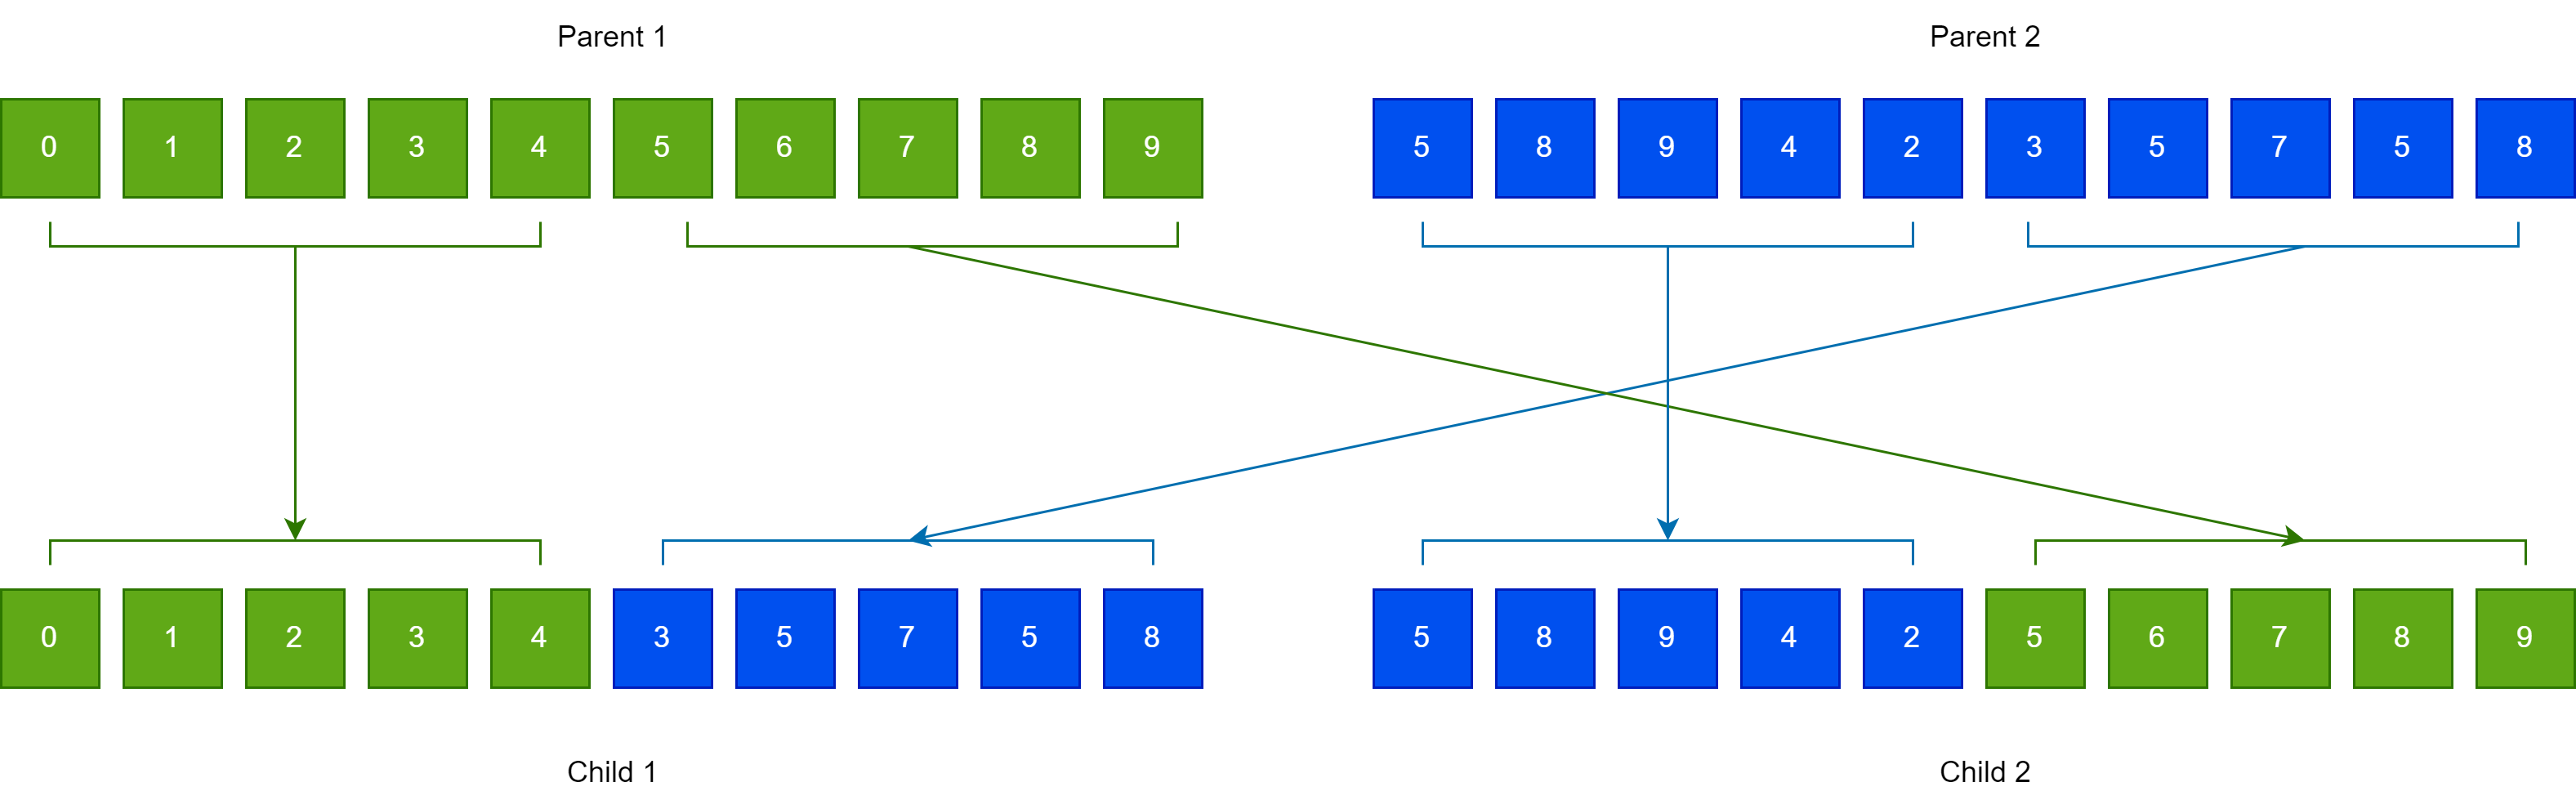
\includegraphics[scale=0.5]{onePointCrossover}
\par\end{centering}
\caption{An example of the method of one - point crossover, used in the Grammatical
Evolution procedure.\label{fig:onePoint}}
\end{figure}
The flowchart for the proposed method is depicted in Figure \ref{fig:flowINNC}.
\begin{figure}[H]
\begin{centering}
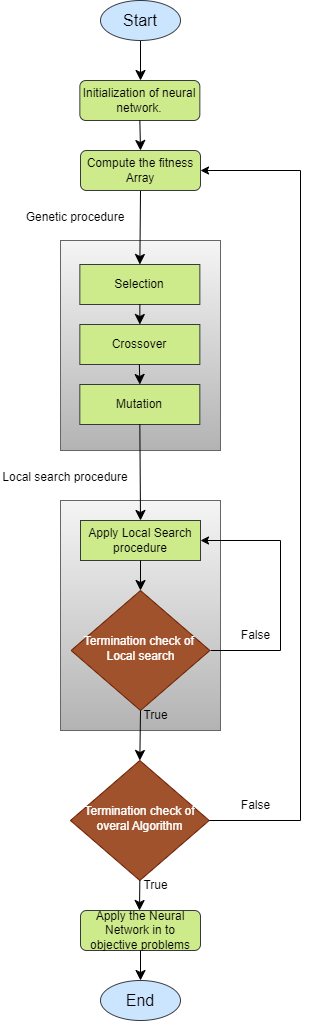
\includegraphics[scale=0.4]{flowchart_innc}
\par\end{centering}
\caption{The flowchart of the proposed algorithm.\label{fig:flowINNC}}

\end{figure}


\subsection{The local search procedure\label{subsec:The-local-search}}

The local search procedure initiates from the vector $\overrightarrow{w}$
that is produced for any given chromosome $g$ using the procedure
described in subsection \ref{subsec:Grammatical-evolution}. The procedure
minimizes the error of equation \ref{eq:eq1} with respect to vector
$\overrightarrow{w}$. The minimization is done within a value interval
created around the initial point $\overrightarrow{w}$ keeping the
network structure intact. The main steps of this procedure are given
below:
\begin{enumerate}
\item \textbf{Set} $d=\left(n+2\right)H$. This value denotes the total
number of parameters for $N\left(\overrightarrow{x},\overrightarrow{w}\right)$.
\item \textbf{For} $i=1,\ldots,d$ \textbf{do}
\begin{enumerate}
\item \textbf{Set} $L_{i}=-F\times\left|w_{i}\right|$, the left bound of
the minimization for the parameter $i$.
\item \textbf{Set} $R_{i}=F\times\left|w_{i}\right|$, the right bound of
the minimization for the parameter $i$.
\end{enumerate}
\item \textbf{EndFor}
\item \textbf{Minimize} the error function of equation \ref{eq:eq1} for
vector $\overrightarrow{w}$ inside the bounding box $\left[\overrightarrow{L},\overrightarrow{R}\right]$
using a local optimization procedure ${\cal L}(w)$. The BFGS method
as modified by Powell \citep{powell} was incorporated in the conducted
experiments.
\end{enumerate}
As an example consider a dataset with $n=2$ and the following constructed
neural network:
\begin{equation}
N\left(\overrightarrow{x},\overrightarrow{w}\right)=2\sigma\left(1.5x_{2}-2.0\right)+2.5\sigma\left(-1.2x_{1}+3.7\right)
\end{equation}
where the number of nodes is $H=2$. In this case the vector $\overrightarrow{w}$
has the elements $\overrightarrow{w}=\left(2,0,1.5,-2,2.5,-1.2,0,3.7\right)$.
If the parameter $F$ has the value $F=2,$then the bound vectors
$\overrightarrow{L}$ and $\overrightarrow{R}$ are defined as:
\begin{eqnarray*}
\overrightarrow{L} & = & \left(-4,0,-3,-4,-5,-2.4,0,7.4\right)\\
\overrightarrow{R} & = & \left(4,0,3,4,5,2.4,0,7.4\right)
\end{eqnarray*}
Hence the minimization method could not change the elements $w_{2}$
and $w_{7}$ and as a consequence the architecture of the network
remains intact.

\section{Experimental results\label{sec:Results}}

The present research work was applied on a series of data classification
and fitting problems, which appeared recently. Also, the proposed
method was compared against other established machine learning methods
from the relevant literature and the results are reported. Furthermore,
a series of experiments were executed to verify the sensitivity of
the proposed technique with respect to the critical parameters presented
earlier.\textbf{ }The following URLs provide the used datasets:
\begin{enumerate}
\item The UCI dataset repository, \url{https://archive.ics.uci.edu/ml/index.php}(accessed
on 28 September 2024)\citep{UCL}
\item The Keel repository, \url{https://sci2s.ugr.es/keel/datasets.php}(accessed
on 28 September 2024)\citep{Keel}.
\item The Statlib URL \url{http://lib.stat.cmu.edu/datasets/ }(accessed
on 28 September 2024). 
\end{enumerate}

\subsection{Classification datasets }

The descriptions of the used datasets are as follows:
\begin{enumerate}
\item \textbf{Appendictis} a medical dataset, originated in \citep{appendicitis}. 
\item \textbf{Australian} dataset \citep{australian}, used in bank transactions.
\item \textbf{Balance} dataset \citep{balance}, that contains data from
psychological experiments.
\item \textbf{Circular} dataset, which is an artificial dataset.
\item \textbf{Cleveland} dataset \citep{cleveland1,cleveland2}.
\item \textbf{Dermatology} dataset \citep{dermatology}, a dataset that
contains measurements about dermatological deceases. 
\item \textbf{Ecoli} dataset, a dataset contains measurements about proteins\citep{ecoli}.
\item \textbf{Fert }dataset, used to detect the relation between sperm concentration
and demographic data.
\item \textbf{Haberman} dataset, a medical dataset related to breast cancer.
\item \textbf{Hayes roth} dataset \citep{hayesroth}, which is related to
a human subjects study.
\item \textbf{Heart} dataset \citep{heart}, a medical dataset used for
the prediction of heart diseases.
\item \textbf{HeartAttack} dataset, used for the detection of heart diseases.
\item \textbf{HouseVotes} dataset \citep{housevotes}. 
\item \textbf{Liverdisorder} dataset \citep{liver}, a medical dataset.
\item \textbf{Ionosphere} dataset, a climate dataset \citep{ion1,ion2}.
\item \textbf{Mammographic} dataset \citep{mammographic}, a dataset related
to the breast cancer.
\item \textbf{Parkinsons} dataset, used in the detection of Parkinson's
disease (PD)\citep{parkinsons}.
\item \textbf{Pima} dataset \citep{pima}, a medical dataset about the detection
of diabetes.
\item \textbf{Popfailures} dataset \citep{popfailures}, a dataset related
to climate measurements.
\item \textbf{Regions2} dataset, used in the detection of hepatitis C \citep{regions}. 
\item \textbf{Saheart} dataset \citep{saheart}, a medical dataset used
for the detection of heart diseases.
\item \textbf{Segment} dataset \citep{segment}, a dataset related to image
processing.
\item \textbf{Spiral} dataset, which is an artificial dataset.
\item \textbf{Student} dataset \citep{student}, which contains data from
experiments conducted in Portuguese schools. 
\item \textbf{Transfusion} dataset\citep{transfusion}, a medical dataset.
\item \textbf{Wdbc} dataset \citep{wdbc}, a dataset related to cancer.
\item \textbf{Wine} dataset, used for the detection of quality of wines.
\citep{wine1,wine2}.
\item \textbf{Eeg} datasets, a medical dataset related to EEG experiments
\citep{eeg}. The following distinct cases were used from this dataset:
Z\_F\_S, Z\_O\_N\_F\_S, ZO\_NF\_S and ZONF\_S.
\item \textbf{Zoo} dataset \citep{zoo}, used for the classification of
animals.
\end{enumerate}
The number of inputs and classes for every classification dataset
is given in Table \ref{tab:patternsClass}.

\begin{table}[H]
\begin{centering}
\begin{tabular}{|c|c|c|}
\hline 
DATASET & INPUTS & CLASSES\tabularnewline
\hline 
\hline 
APPENDICITIS & 7 & 2\tabularnewline
\hline 
AUSTRALIAN & 14 & 2\tabularnewline
\hline 
BALANCE & 4 & 3\tabularnewline
\hline 
CIRCULAR & 5 & 2\tabularnewline
\hline 
CLEVELAND & 13 & 5\tabularnewline
\hline 
DERMATOLOGY & 34 & 6\tabularnewline
\hline 
ECOLI & 7 & 8\tabularnewline
\hline 
FERT & 9 & 2\tabularnewline
\hline 
HABERMAN & 3 & 2\tabularnewline
\hline 
HAYES ROTH & 5 & 3\tabularnewline
\hline 
HEART & 13 & 2\tabularnewline
\hline 
HEART ATTACK & 13 & 2\tabularnewline
\hline 
HOUSEVOTES & 16 & 2\tabularnewline
\hline 
LIVERDISORDER & 6 & 2\tabularnewline
\hline 
IONOSPHERE & 34 & 2\tabularnewline
\hline 
MAMMOGRAPHIC & 5 & 2\tabularnewline
\hline 
PARKINSONS & 22 & 2\tabularnewline
\hline 
PIMA & 8 & 2\tabularnewline
\hline 
POPFAILURES & 18 & 2\tabularnewline
\hline 
REGIONS2 & 18 & 5\tabularnewline
\hline 
SAHEART & 9 & 2\tabularnewline
\hline 
SEGMENT & 19 & 7\tabularnewline
\hline 
SPIRAL & 2 & 2\tabularnewline
\hline 
STUDENT & 5 & 4\tabularnewline
\hline 
TRANSFUSION & 4 & 2\tabularnewline
\hline 
WDBC & 30 & 2\tabularnewline
\hline 
WINE & 13 & 3\tabularnewline
\hline 
Z\_F\_S & 21 & 3\tabularnewline
\hline 
Z\_O\_N\_F\_S & 21 & 5\tabularnewline
\hline 
ZO\_NF\_S & 21 & 3\tabularnewline
\hline 
ZONF\_S & 21 & 2\tabularnewline
\hline 
ZOO & 16 & 7\tabularnewline
\hline 
\end{tabular}
\par\end{centering}
\caption{Number of inputs and distinct classes for every classification dataset.\label{tab:patternsClass}}

\end{table}


\subsection{Regression datasets }

The description for the incorporated regression datasets is given
below:
\begin{enumerate}
\item \textbf{Abalone} dataset \citep{abalone}, used to predict the age
of abalones.
\item \textbf{Airfoil }dataset, a dataset provided by NASA \citep{airfoil}.
\item \textbf{BK} dataset \citep{Stat}, used to predict the points scored
in a basketball game. 
\item \textbf{BL} dataset, related to an electricity experiment.
\item \textbf{Baseball} dataset, used to predict the average income of baseball
players.
\item \textbf{Concrete} dataset \citep{concrete}, which is a civil engineering
dataset.
\item \textbf{Dee} dataset, that contains measurements about the price of
electricity.
\item \textbf{FY, }this dataset used to measure the longevity of fruit flies. 
\item \textbf{HO} dataset, downloaded from the STALIB repository.
\item \textbf{Housing} dataset, originated in \citep{housing}.
\item \textbf{Laser} dataset, that contains data from laser experiments
\item \textbf{LW} dataset, related to risk factors associated with low weight
babies.
\item \textbf{MORTGAGE} dataset, an economic dataset.
\item \textbf{MUNDIAL, }downloaded from the STALIB repository.
\item \textbf{PL} dataset, downloaded from the STALIB repository.
\item \textbf{QUAKE} dataset, contains data about the strength of a earthquakes.
\item \textbf{REALESTATE, }downloaded from the STALIB repository.
\item \textbf{SN} dataset, that contains measurements from an experiment
related to trellising and pruning. 
\item \textbf{Treasury} dataset, an economic dataset.
\item \textbf{VE} dataset, downloaded from the STALIB repository.
\item \textbf{TZ} dataset, downloaded from the STALIB repository.
\end{enumerate}
The number of inputs for each dataset is provided in Table \ref{tab:inputsRegression}.

\begin{table}[H]

\caption{Number of inputs for every regression dataset.\label{tab:inputsRegression}}

\centering{}%
\begin{tabular}{|c|c|}
\hline 
DATASET & INPUTS\tabularnewline
\hline 
\hline 
ABALONE & 8\tabularnewline
\hline 
AIRFOIL & 5\tabularnewline
\hline 
BASEBALL & 16\tabularnewline
\hline 
BK & 4\tabularnewline
\hline 
BL & 7\tabularnewline
\hline 
CONCRETE & 8\tabularnewline
\hline 
DEE & 6\tabularnewline
\hline 
HO & 13\tabularnewline
\hline 
HOUSING & 13\tabularnewline
\hline 
FY & 4\tabularnewline
\hline 
LASER & 4\tabularnewline
\hline 
LW & 9\tabularnewline
\hline 
MORTGAGE & 15\tabularnewline
\hline 
MUNDIAL & 3\tabularnewline
\hline 
PL & 2\tabularnewline
\hline 
QUAKE & 3\tabularnewline
\hline 
REALESTATE & 5\tabularnewline
\hline 
SN & 11\tabularnewline
\hline 
TREASURY & 15\tabularnewline
\hline 
TZ & 60\tabularnewline
\hline 
VE & 7\tabularnewline
\hline 
\end{tabular}
\end{table}


\subsection{Experimental results}

The code used in the experiments was written in ANSI C++ using the
optimization environment of Optimus, which is freely available from
\url{https://github.com/itsoulos/GlobalOptimus/}( accessed on 28
September 2024 ). All the experiments were conducted and averages
were recorded. In every execution, a different seed for the random
generator was used. The average classification error as measured on
the test is recorded for the classification datasets and the average
regression error for the regression datasets. For the case of classification
datasets the displayed classification error for a model $M(x)$ and
the test dataset $T$ is calculated as:
\begin{equation}
E_{C}\left(M(x)\right)=100\times\frac{\sum_{i=1}^{N}\left(\mbox{class}\left(M\left(x_{i}\right)\right)-y_{i}\right)}{N}
\end{equation}
The test set $T$ is defined as $T=\left(x_{i},y_{i}\right),\ i=1,\ldots,N$
For the case of regression problems the regression error $E_{R}\left(M(x)\right)$
is defined as:
\begin{equation}
E_{R}\left(M(x)\right)=\frac{\sum_{i=1}^{N}\left(M\left(x_{i}\right)-y_{i}\right)^{2}}{N}
\end{equation}
The validation of the conducted experiments was performed using the
ten - fold cross validation technique.  The experiments were carried
out on an AMD Ryzen 5950X with 128GB of RAM, running the Debian Linux
operating system. The values for the parameters of the algorithms
are shown in  Table \ref{tab:experSettings}. In all experimental
tables, the bold notation is used to mark the method with the lowest
classification or regression error.

\begin{table}[H]
\caption{The values used in the experimental parameters.\label{tab:experSettings}}

\centering{}%
\begin{tabular}{|c|c|c|}
\hline 
PARAMETER & MEANING & VALUE\tabularnewline
\hline 
\hline 
$N_{c}$ & Number of chromosomes & 500\tabularnewline
\hline 
$N_{g}$ & Maximum number of generations & 200\tabularnewline
\hline 
$p_{s}$ & Crossover rate & 0.10\tabularnewline
\hline 
$p_{m}$ & Mutation rate & 0.05\tabularnewline
\hline 
$N_{T}$ & Number of chromosomes that selected randomly & 20\tabularnewline
\hline 
$N_{I}$ & Number of iterations before local search & 10\tabularnewline
\hline 
$F$ & Magnitude of changes from local search & 4.0\tabularnewline
\hline 
\end{tabular}
\end{table}
Table \ref{tab:classResults} contains the experimental results for
the classification datasets and Table \ref{tab:resultsRegression}
the experimental results for the regression datasets. The neural network
used in the experimental results has one processing unit with $H=10$
processing nodes and the sigmoid function as activation function.
The following notation was used in these tables:
\begin{enumerate}
\item The column BFGS represents the application of the BFGS method. This
method was used to train an artificial neural network with $H=10$
processing nodes.
\item The column GENETIC stands for the incorporation of a Genetic Algorithm
to train a neural network with $H=10$ processing nodes. This genetic
algorithm uses the values of Table \ref{tab:experSettings}.
\item The column NNC stands for the usage of the original neural network
construction model to the provided dataset.
\item The column INNC stands for the incorporation of the current work to
the provided dataset.
\item The row AVERAGE contains the average classification or regression
error, as measured on all datasets.
\end{enumerate}
The methods BFGS and GENETIC train the neural network $N\left(\overrightarrow{x},\overrightarrow{w}\right)$
by minimizing the error function defined in Equation \ref{eq:eq1}.
\begin{table}[H]
\caption{Results from the application of machine learning models on the classification
datasets. Numbers in cells represent average classification error
for the corresponding test set.\label{tab:classResults}}

\centering{}%
\begin{tabular}{|c|c|c|c|c|}
\hline 
\textbf{DATASET} & \textbf{BFGS} & \textbf{GENETIC} & \textbf{NNC} & \textbf{INNC}\tabularnewline
\hline 
\hline 
APPENDICITIS & 18.00\% & 24.40\% & \textbf{13.70\%} & 14.70\%\tabularnewline
\hline 
AUSTRALIAN & 38.13\% & 36.64\% & \textbf{14.51\%} & 14.80\%\tabularnewline
\hline 
BALANCE & 8.64\% & \textbf{8.36\%} & 22.11\% & 8.66\%\tabularnewline
\hline 
CIRCULAR & 6.08\% & \textbf{5.13\%} & 13.64\% & 5.32\%\tabularnewline
\hline 
CLEVELAND & 77.55\% & 57.21\% & 50.10\% & \textbf{47.93\%}\tabularnewline
\hline 
DERMATOLOGY & 52.92\% & \textbf{16.60\%} & 25.06\% & 20.89\%\tabularnewline
\hline 
ECOLI & 69.52\% & 54.67\% & \textbf{47.82\%} & 48.21\%\tabularnewline
\hline 
FERT & 23.20\% & 28.50\% & \textbf{19.00\%} & 20.50\%\tabularnewline
\hline 
HABERMAN & 29.34\% & 28.66\% & 28.03\% & \textbf{26.70\%}\tabularnewline
\hline 
HAYES-ROTH & 37.33\% & 56.18\% & 35.93\% & \textbf{31.77\%}\tabularnewline
\hline 
HEART & 39.44\% & 26.41\% & 15.78\% & \textbf{14.74\%}\tabularnewline
\hline 
HEARTATTACK & 46.67\% & 29.03\% & \textbf{19.33\%} & 20.43\%\tabularnewline
\hline 
HOUSEVOTES & 7.13\% & 7.00\% & 3.65\% & \textbf{3.26\%}\tabularnewline
\hline 
IONOSPHERE & 15.29\% & 15.14\% & \textbf{11.12\%} & 11.92\%\tabularnewline
\hline 
LIVERDISORDER & 42.59\% & 37.09\% & 33.71\% & \textbf{31.77\%}\tabularnewline
\hline 
MAMMOGRAPHIC & 17.24\% & 19.88\% & 17.78\% & \textbf{15.81\%}\tabularnewline
\hline 
PARKINSONS & 27.58\% & 16.58\% & \textbf{12.21\%} & 12.53\%\tabularnewline
\hline 
PIMA & 35.59\% & 34.21\% & 27.99\% & \textbf{24.00\%}\tabularnewline
\hline 
POPFAILURES & 5.24\% & \textbf{4.17\%} & 6.74\% & 6.44\%\tabularnewline
\hline 
REGIONS2 & 36.28\% & 33.53\% & 25.52\% & \textbf{23.18\%}\tabularnewline
\hline 
SAHEART & 37.48\% & 34.85\% & 30.52\% & \textbf{28.09\%}\tabularnewline
\hline 
SEGMENT & 68.97\% & 46.30\% & 54.99\% & \textbf{43.12\%}\tabularnewline
\hline 
SPIRAL & 47.99\% & 47.67\% & 48.39\% & \textbf{43.99\%}\tabularnewline
\hline 
STUDENT & 7.14\% & 5.61\% & 5.78\% & \textbf{4.55\%}\tabularnewline
\hline 
TRANSFUSION & 25.80\% & 25.84\% & 25.34\% & \textbf{23.43\%}\tabularnewline
\hline 
WDBC & 29.91\% & 7.87\% & 6.95\% & \textbf{4.41\%}\tabularnewline
\hline 
WINE & 59.71\% & 22.88\% & 14.35\% & \textbf{9.77\%}\tabularnewline
\hline 
Z\_F\_S & 39.37\% & 24.60\% & 14.17\% & \textbf{8.53\%}\tabularnewline
\hline 
Z\_O\_N\_F\_S & 65.67\% & 64.81\% & 49.18\% & \textbf{38.58\%}\tabularnewline
\hline 
ZO\_NF\_S & 43.04\% & 21.54\% & 14.14\% & \textbf{6.84\%}\tabularnewline
\hline 
ZONF\_S & 15.62\% & 4.36\% & 3.14\% & \textbf{2.52\%}\tabularnewline
\hline 
ZOO & 10.70\% & 9.50\% & 9.20\% & \textbf{7.20\%}\tabularnewline
\hline 
\textbf{AVERAGE} & \textbf{33.91\%} & \textbf{26.73\%} & \textbf{22.50\%} & \textbf{19.52\%}\tabularnewline
\hline 
\end{tabular}
\end{table}
\begin{table}[H]
\caption{Results from the conducted experiments on the regression datasets.
Numbers in cells denote average regression error as calculated on
the corresponding test set.\label{tab:resultsRegression}}

\centering{}%
\begin{tabular}{|c|c|c|c|c|}
\hline 
\textbf{DATASET} & \textbf{BFGS} & \textbf{GENETIC} & \textbf{NNC} & \textbf{INNC}\tabularnewline
\hline 
\hline 
ABALONE & 5.69 & 7.17 & 5.05 & \textbf{4.33}\tabularnewline
\hline 
AIRFOIL & 0.003 & 0.003 & 0.003 & \textbf{0.002}\tabularnewline
\hline 
BASEBALL & 119.63 & 64.60 & 59.85 & \textbf{48.42}\tabularnewline
\hline 
BK & 0.36 & 0.26 & 2.32 & \textbf{0.07}\tabularnewline
\hline 
BL & 1.09 & 2.23 & 0.021 & \textbf{0.002}\tabularnewline
\hline 
CONCRETE & 0.066 & 0.01 & 0.008 & \textbf{0.005}\tabularnewline
\hline 
DEE & 2.36 & 1.01 & 0.26 & \textbf{0.23}\tabularnewline
\hline 
HO & 0.62 & 0.37 & 0.017 & \textbf{0.01}\tabularnewline
\hline 
HOUSING & 97.38 & 43.26 & 26.35 & \textbf{16.01}\tabularnewline
\hline 
FY & 0.19 & 0.65 & 0.058 & \textbf{0.042}\tabularnewline
\hline 
LASER & 0.015 & 0.59 & 0.024 & \textbf{0.005}\tabularnewline
\hline 
LW & 2.98 & 0.54 & \textbf{0.011} & 0.012\tabularnewline
\hline 
MORTGAGE & 8.23 & 0.40 & 0.30 & \textbf{0.026}\tabularnewline
\hline 
MUNDIAL & 6.48 & 1.22 & 4.47 & \textbf{0.034}\tabularnewline
\hline 
PL & 0.29 & 0.28 & 0.045 & \textbf{0.022}\tabularnewline
\hline 
QUAKE & 0.42 & 0.12 & 0.045 & \textbf{0.04}\tabularnewline
\hline 
REALESTATE & 128.94 & 81.19 & 76.78 & \textbf{70.99}\tabularnewline
\hline 
SN & 3.89 & 0.40 & 0.026 & \textbf{0.023}\tabularnewline
\hline 
TREASURY & 9.91 & 2.93 & 0.47 & \textbf{0.066}\tabularnewline
\hline 
TZ & 3.27 & 5.38 & 5.04 & \textbf{0.03}\tabularnewline
\hline 
VE & 1.92 & 2.43 & 6.61 & \textbf{0.025}\tabularnewline
\hline 
\textbf{AVERAGE} & \textbf{18.75} & \textbf{10.24} & \textbf{8.94} & \textbf{6.69}\tabularnewline
\hline 
\end{tabular}
\end{table}
The original technique of constructing artificial neural networks
has significantly lower classification or regression errors than the
other two techniques and the proposed method significantly improves
the performance of this technique in the majority of the datasets.
The percentage improvement in error is even greater in regression
problems. In some cases the improvement exceeds 50\% in the test error.
This effect is evident in the box plots for classification and regression
errors outlined in Figures \ref{fig:boxClass} and \ref{fig:boxRegression}
respectively.

\begin{figure}[H]
\begin{centering}
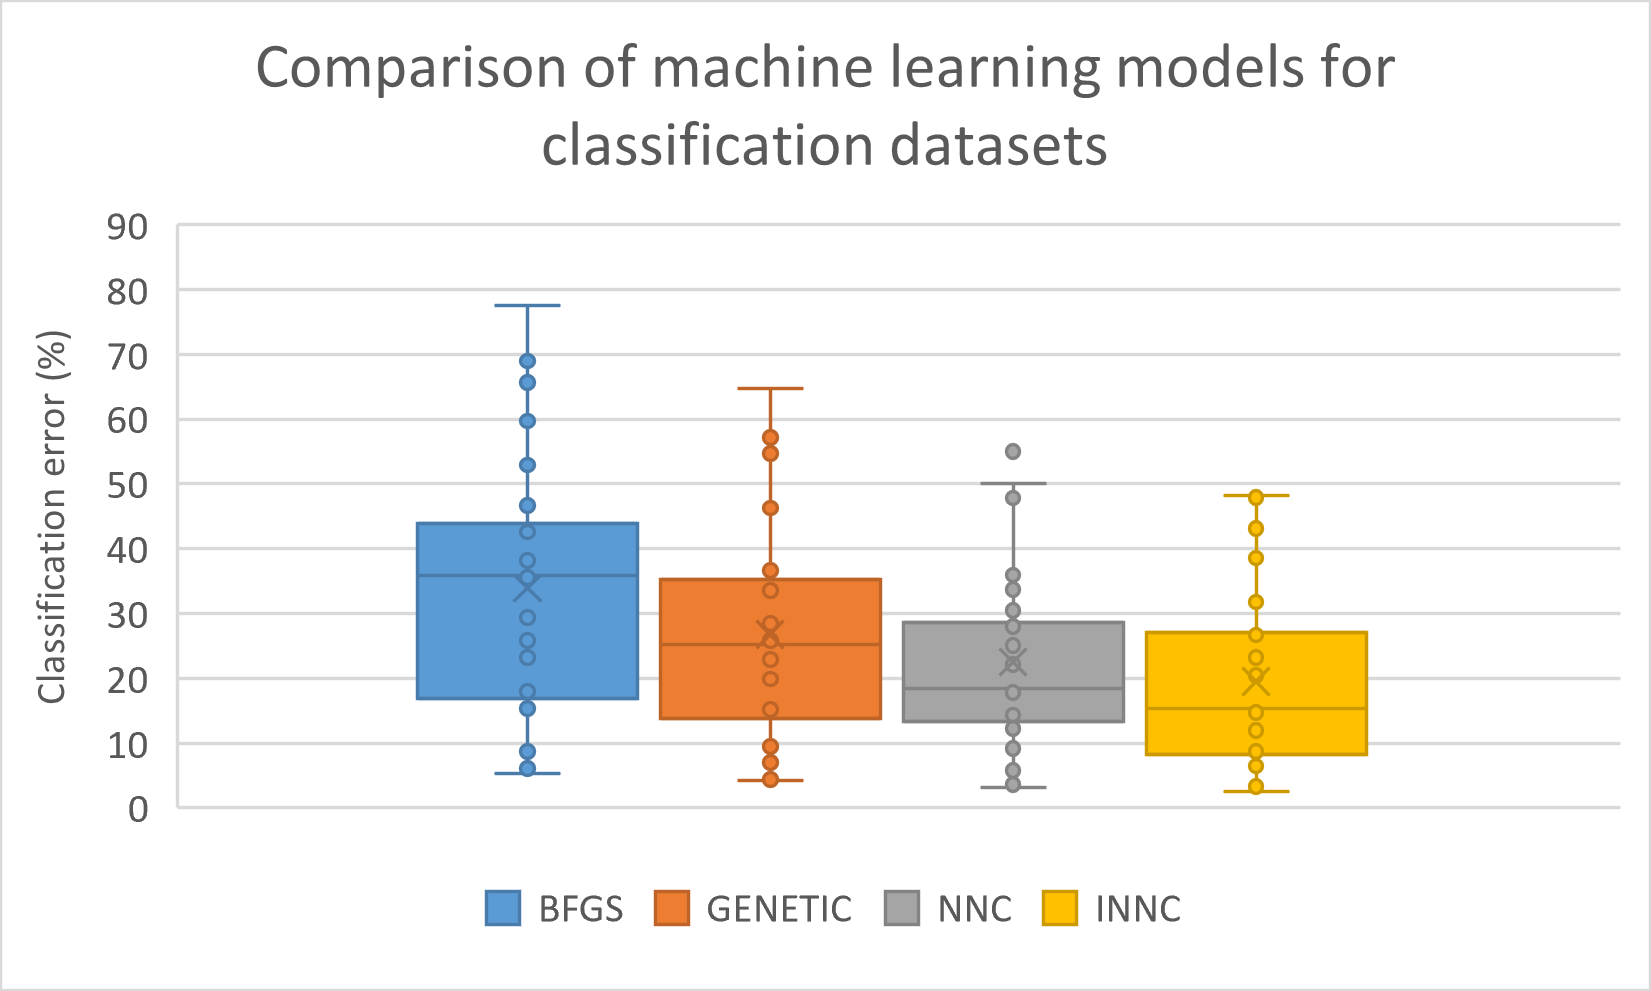
\includegraphics{table1}
\par\end{centering}
\caption{Box plot for the comparison between the machine learning methods applied
on the classification datasets.\label{fig:boxClass}}

\end{figure}
\begin{figure}[H]
\begin{centering}
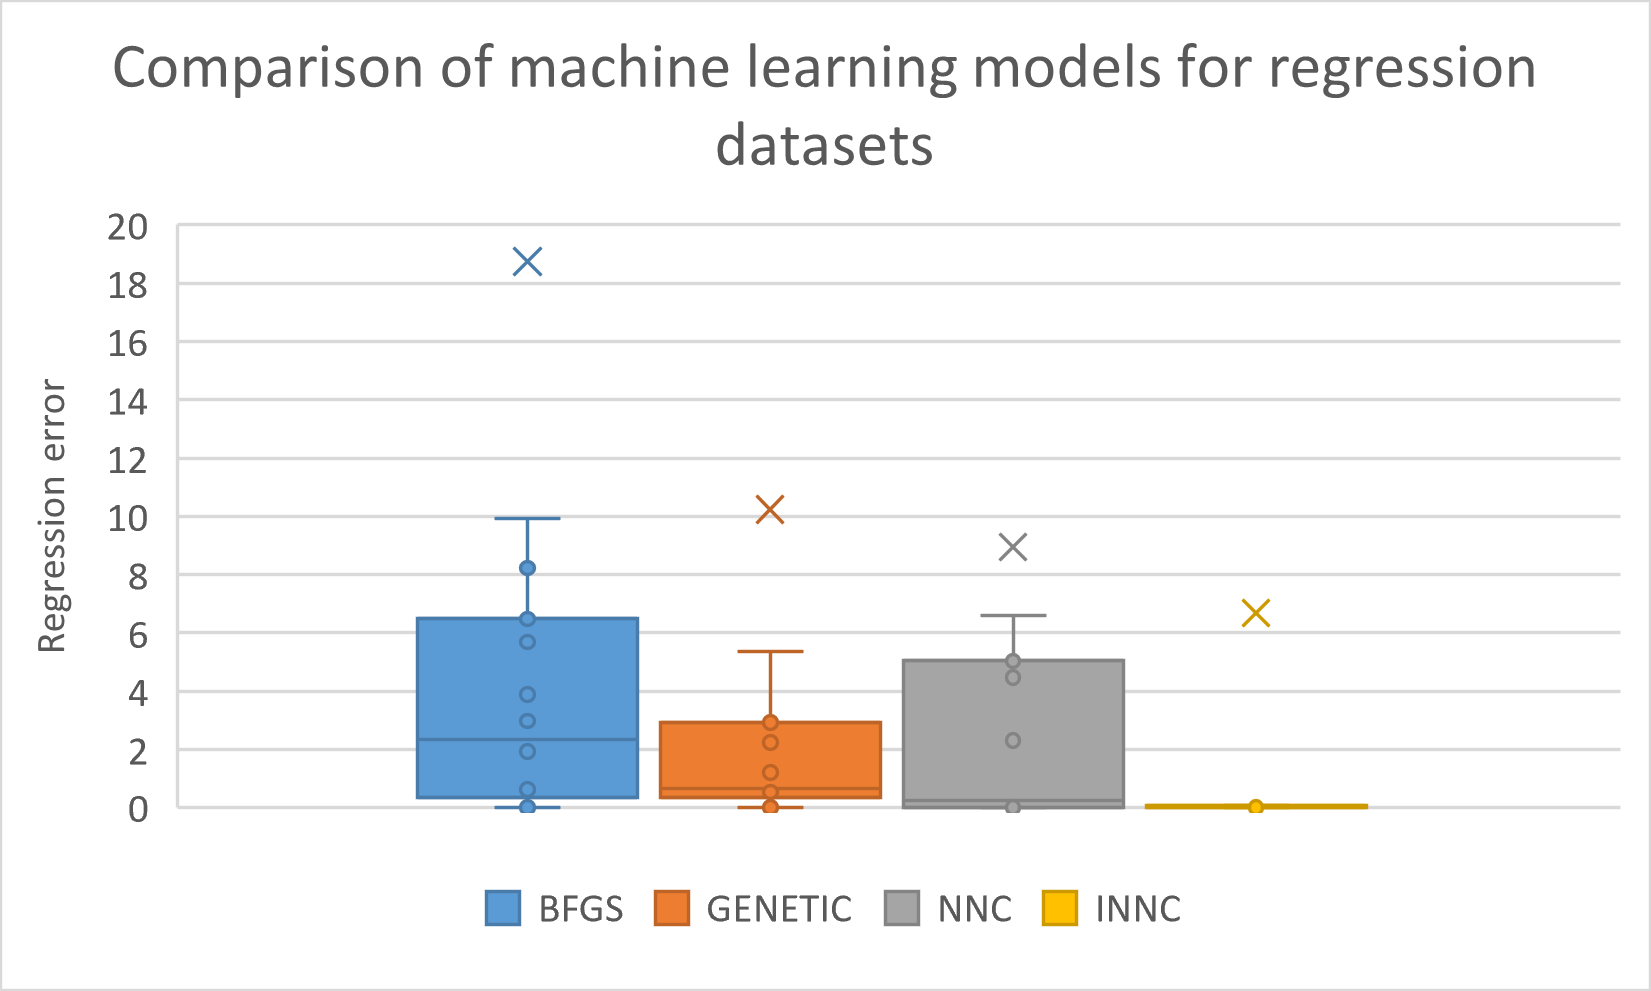
\includegraphics{table2}
\par\end{centering}
\caption{Box plot for the comparison between the machine learning methods applied
on the regression datasets.\label{fig:boxRegression}}
\end{figure}
Furthermore, the same reduction in test error is validated from the
statistical tests performed for classification and regression problems.
These tests are depicted in Figures \ref{fig:statisticsClass} and
\ref{fig:statRegression}.

\begin{figure}[H]
\begin{centering}
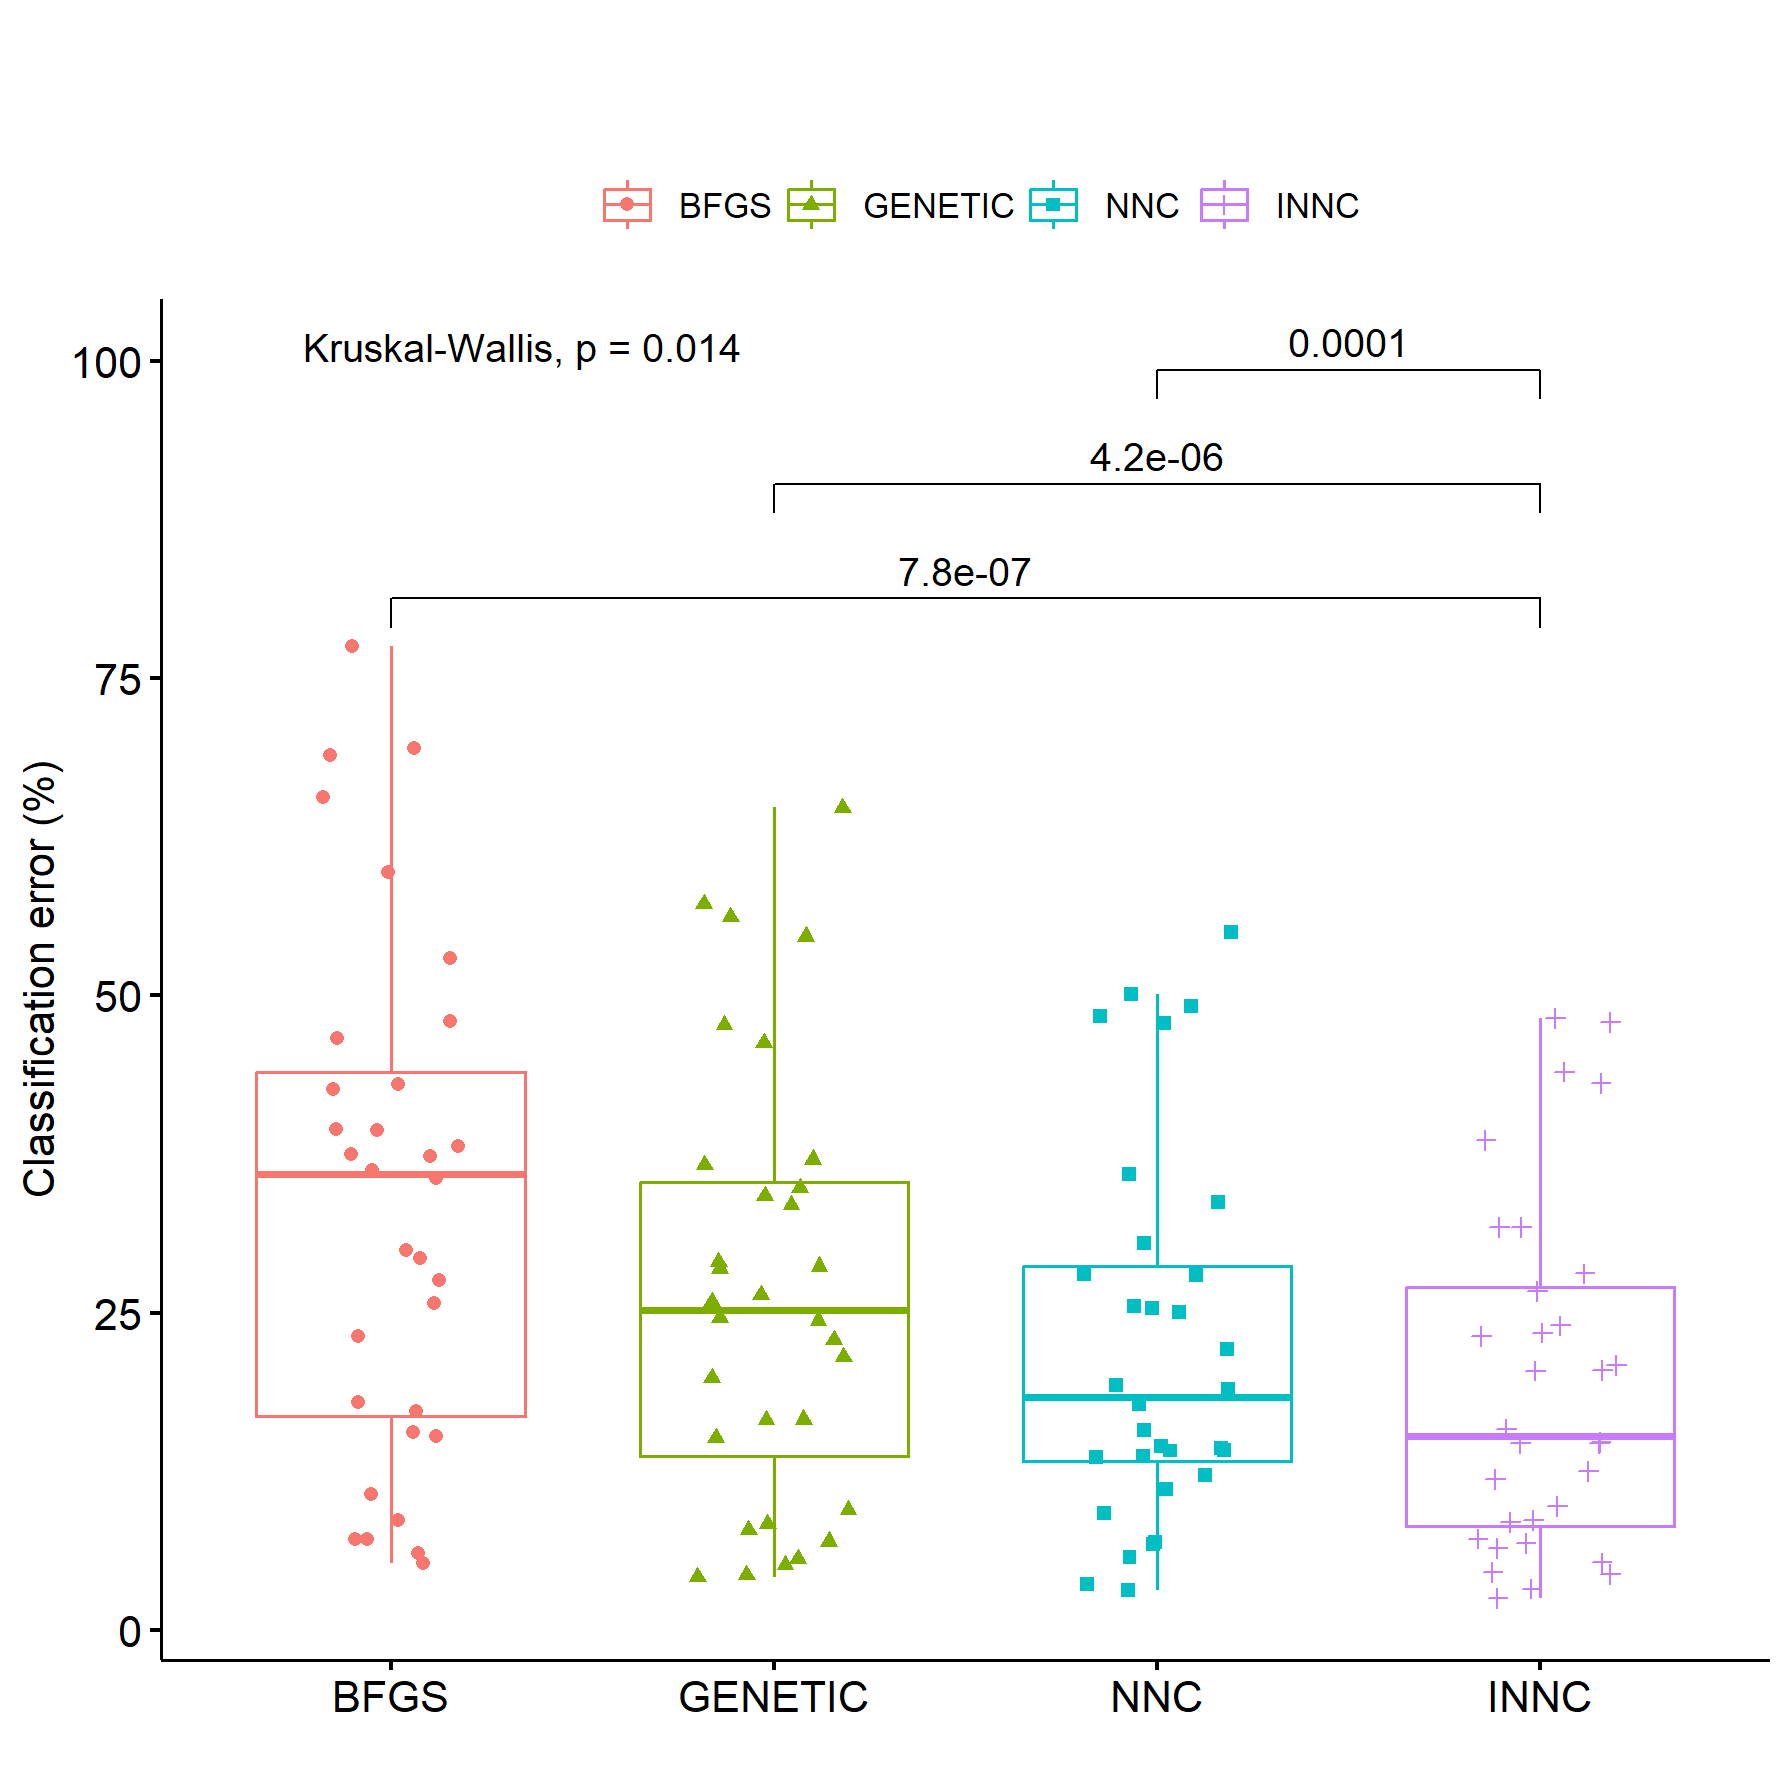
\includegraphics[scale=0.6]{table1_stat}
\par\end{centering}
\caption{Statistical test for all machine learning models that was applied
on the classification datasets.\label{fig:statisticsClass}}
\end{figure}
\begin{figure}[H]
\begin{centering}
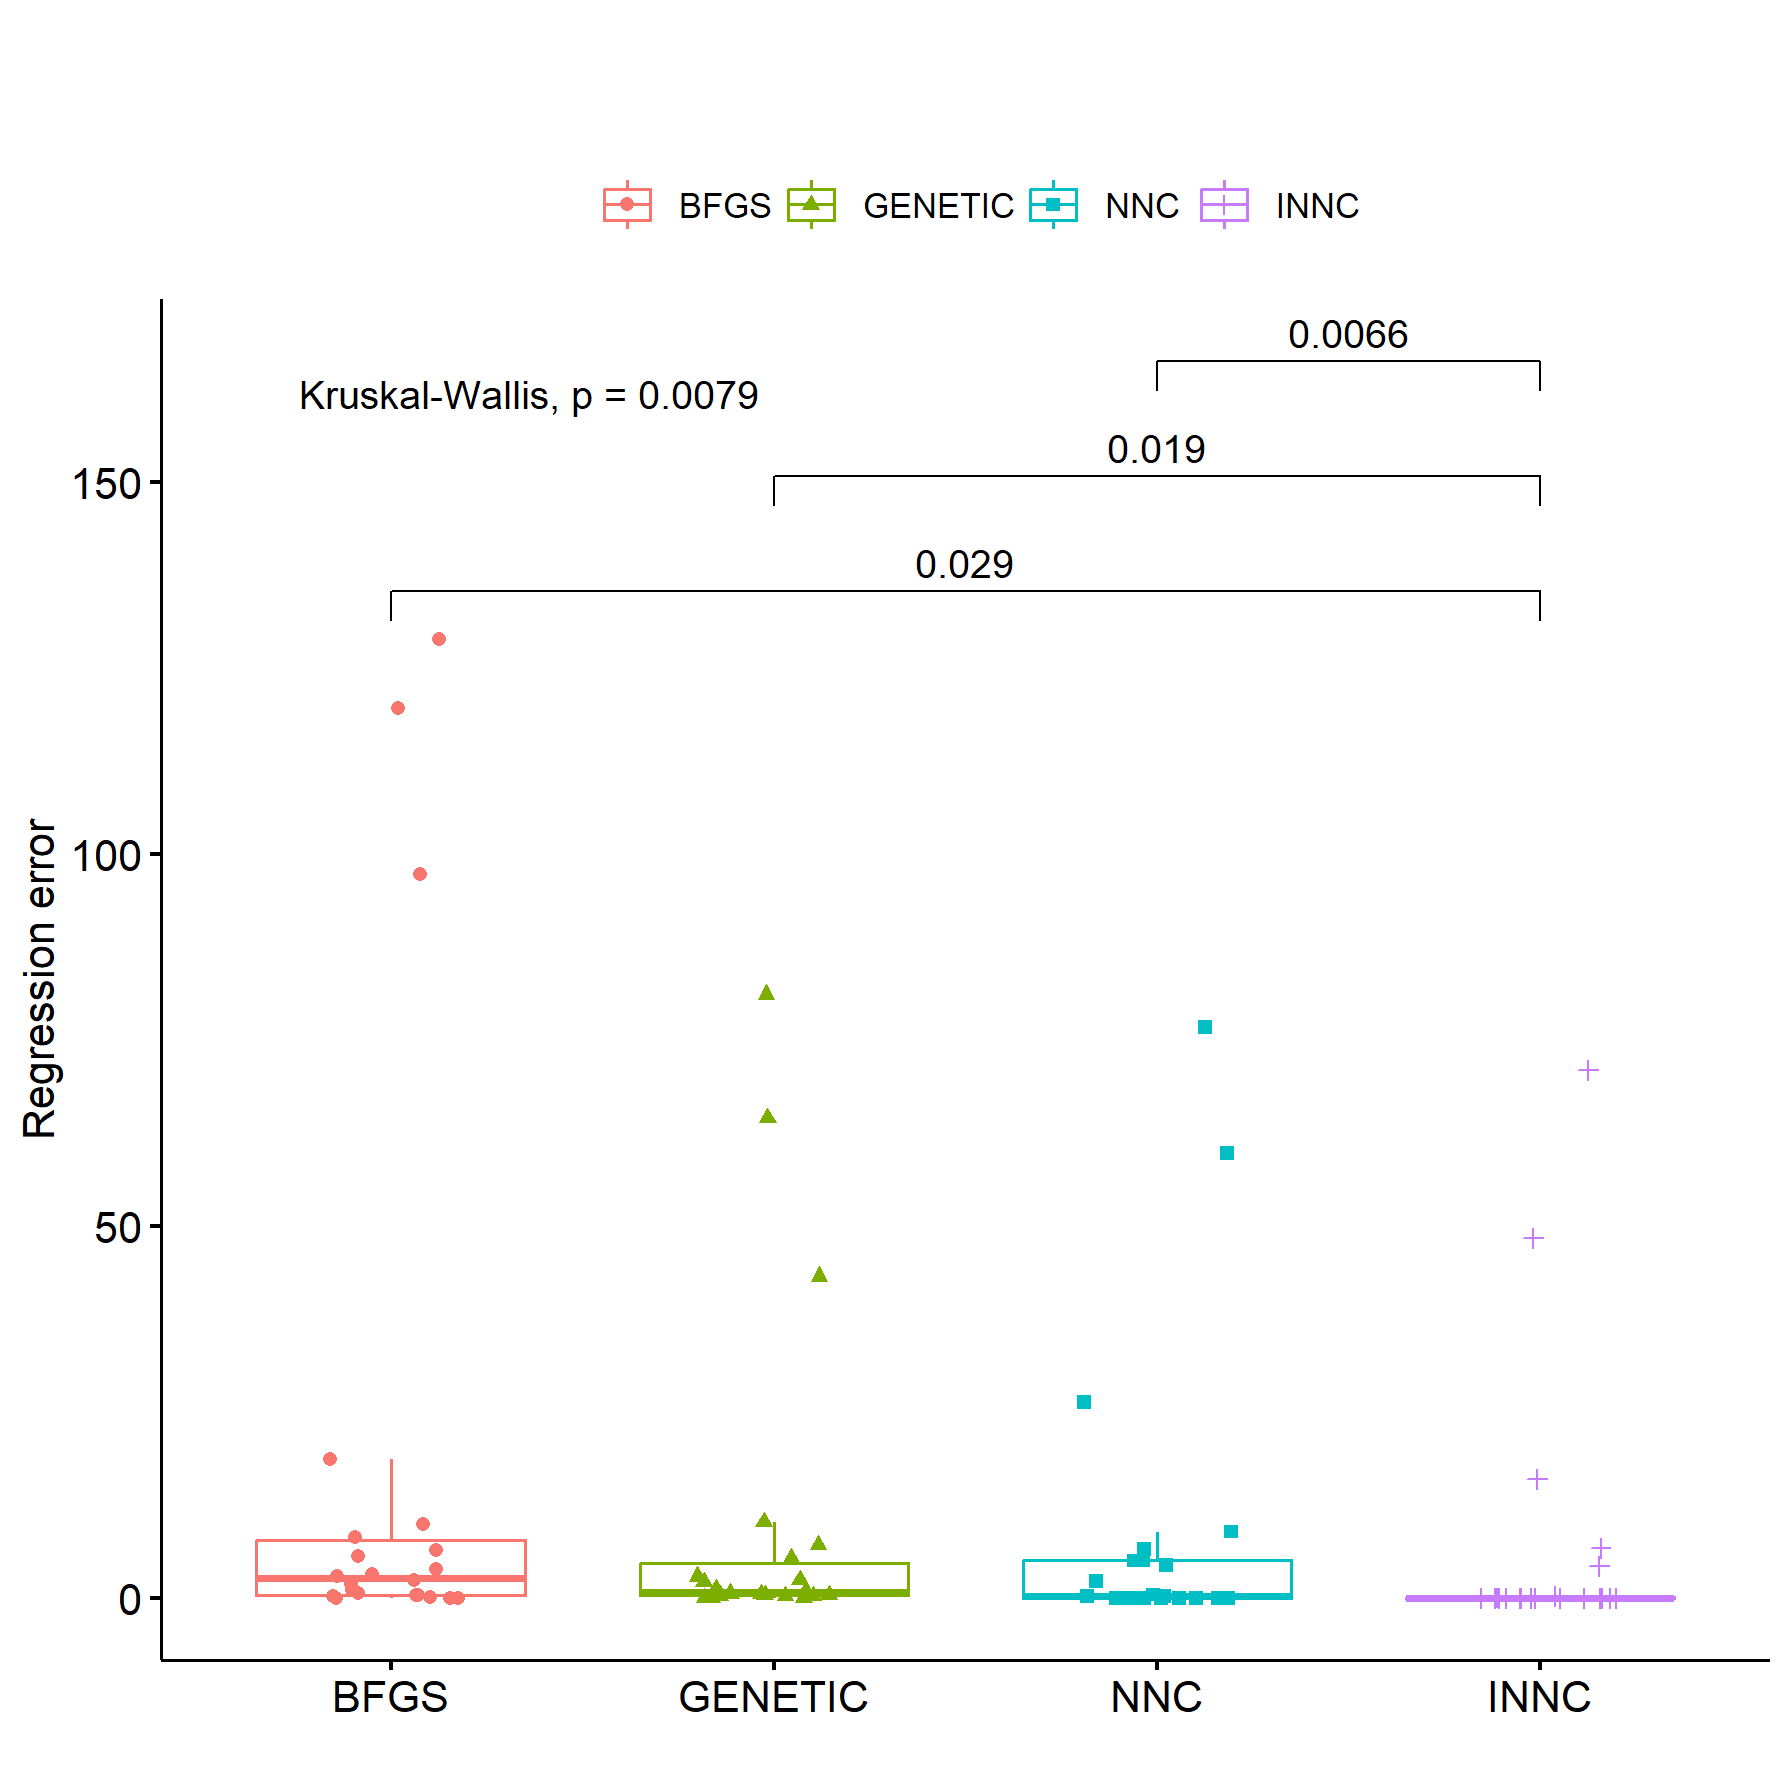
\includegraphics[scale=0.6]{table2_stat}
\par\end{centering}
\caption{Statistical test for all machine learning models that was applied
on the regression datasets.\label{fig:statRegression}}

\end{figure}


\subsubsection{Experiments with the parameter $N_{I}$}

To verify the robustness of the proposed technique as well as its
sensitivity to parameter changes, an additional experiment was performed
in which the critical $N_{I}$ parameter was varied from 5 to 20.
This parameter determines the number of generations intervening before
the local optimization method is executed on randomly selected chromosomes.
The results from this experiment for the classification datasets are
depicted in Table \ref{tab:experRClass} and the results for the regression
datasets in Table \ref{tab:experRRegression}.

\begin{table}[H]
\caption{Experimental results with different values for the parameter $N_{I}$
of the proposed method. The method was applied on the classification
datasets.\label{tab:experRClass}}

\centering{}%
\begin{tabular}{|c|c|c|c|}
\hline 
\textbf{DATASET} & \textbf{INNC$\left(N_{I}=5\right)$} & \textbf{INNC$\left(N_{I}=10\right)$} & \textbf{INNC$\left(N_{I}=20\right)$}\tabularnewline
\hline 
\hline 
APPENDICITIS & 14.50\% & 14.70\% & \textbf{14.20\%}\tabularnewline
\hline 
AUSTRALIAN & \textbf{14.48\%} & 14.80\% & 14.58\%\tabularnewline
\hline 
BALANCE & \textbf{7.63\%} & 8.66\% & 11.71\%\tabularnewline
\hline 
CIRCULAR & \textbf{5.25\%} & 5.32\% & 5.87\%\tabularnewline
\hline 
CLEVELAND & 48.41\% & \textbf{47.93\%} & 49.66\%\tabularnewline
\hline 
DERMATOLOGY & \textbf{19.66\%} & 20.89\% & 23.11\%\tabularnewline
\hline 
ECOLI & \textbf{47.39\%} & 48.21\% & 48.09\%\tabularnewline
\hline 
FERT & 20.80\% & \textbf{20.50\%} & 20.90\%\tabularnewline
\hline 
HABERMAN & 26.87\% & \textbf{26.70\%} & 27.27\%\tabularnewline
\hline 
HAYES-ROTH & \textbf{31.69\%} & 31.77\% & 35.92\%\tabularnewline
\hline 
HEART & 14.85\% & \textbf{14.74\%} & 15.56\%\tabularnewline
\hline 
HEARTATTACK & 20.10\% & 20.43\% & \textbf{20.07\%}\tabularnewline
\hline 
HOUSEVOTES & 3.87\% & \textbf{3.26\%} & 3.78\%\tabularnewline
\hline 
IONOSPHERE & 11.51\% & 11.92\% & \textbf{11.09\%}\tabularnewline
\hline 
LIVERDISORDER & \textbf{31.35\%} & 31.77\% & 31.85\%\tabularnewline
\hline 
MAMMOGRAPHIC & 16.25\% & \textbf{15.81\%} & 16.06\%\tabularnewline
\hline 
PARKINSONS & 13.16\% & \textbf{12.53\%} & 12.58\%\tabularnewline
\hline 
PIMA & \textbf{23.95\%} & 24.00\% & 24.67\%\tabularnewline
\hline 
POPFAILURES & \textbf{6.06\%} & 6.44\% & 6.48\%\tabularnewline
\hline 
REGIONS2 & 23.36\% & \textbf{23.18\%} & 24.21\%\tabularnewline
\hline 
SAHEART & \textbf{27.68\%} & 28.09\% & 29.41\%\tabularnewline
\hline 
SEGMENT & 43.79\% & \textbf{43.12\%} & 46.91\%\tabularnewline
\hline 
SPIRAL & \textbf{43.63\%} & 43.99\% & 45.15\%\tabularnewline
\hline 
STUDENT & \textbf{3.65\%} & 4.55\% & 3.88\%\tabularnewline
\hline 
TRANSFUSION & \textbf{22.62\%} & 23.43\% & 23.89\%\tabularnewline
\hline 
WDBC & \textbf{4.41\%} & 4.41\% & 5.46\%\tabularnewline
\hline 
WINE & 10.18\% & \textbf{9.77\%} & 12.00\%\tabularnewline
\hline 
Z\_F\_S & \textbf{7.70\%} & 8.53\% & 9.63\%\tabularnewline
\hline 
Z\_O\_N\_F\_S & \textbf{36.64\%} & 38.58\% & 41.08\%\tabularnewline
\hline 
ZO\_NF\_S & \textbf{6.84\%} & 6.84\% & 6.90\%\tabularnewline
\hline 
ZONF\_S & \textbf{2.24\%} & 2.52\% & 2.66\%\tabularnewline
\hline 
ZOO & \textbf{6.30\%} & 7.20\% & 7.70\%\tabularnewline
\hline 
\textbf{AVERAGE} & \textbf{19.28\%} & \textbf{19.52\%} & \textbf{20.39\%}\tabularnewline
\hline 
\end{tabular}
\end{table}
\begin{table}[H]
\caption{Experimental results with a variety of values for the parameter $N_{I}$.
The current work was applied on the regression datasets.\label{tab:experRRegression}}

\centering{}%
\begin{tabular}{|c|c|c|c|}
\hline 
\textbf{DATASET} & \textbf{INNC}$\left(N_{I}=5\right)$ & \textbf{INNC$\left(N_{I}=10\right)$} & \textbf{INNC}$\left(N_{I}=20\right)$\tabularnewline
\hline 
\hline 
ABALONE & 4.38 & \textbf{4.33} & 4.45\tabularnewline
\hline 
AIRFOIL & 0.002 & \textbf{0.002} & 0.002\tabularnewline
\hline 
BASEBALL & \textbf{47.50} & 48.42 & 49.99\tabularnewline
\hline 
BK & 0.64 & \textbf{0.07} & 1.86\tabularnewline
\hline 
BL & 0.014 & \textbf{0.002} & 0.003\tabularnewline
\hline 
CONCRETE & \textbf{0.005} & 0.005 & 0.005\tabularnewline
\hline 
DEE & \textbf{0.22} & 0.23 & 0.23\tabularnewline
\hline 
HO & \textbf{0.01} & 0.01 & 0.011\tabularnewline
\hline 
HOUSING & 21.09 & \textbf{16.01} & 16.96\tabularnewline
\hline 
FY & 0.046 & \textbf{0.042} & 0.19\tabularnewline
\hline 
LASER & \textbf{0.004} & 0.005 & 0.005\tabularnewline
\hline 
LW & \textbf{0.011} & 0.012 & 0.011\tabularnewline
\hline 
MORTGAGE & \textbf{0.02} & 0.026 & 0.03\tabularnewline
\hline 
MUNDIAL & 0.031 & 0.034 & \textbf{0.029}\tabularnewline
\hline 
PL & \textbf{0.022} & 0.022 & 0.022\tabularnewline
\hline 
QUAKE & 0.045 & 0.04 & \textbf{0.037}\tabularnewline
\hline 
REALESTATE & \textbf{68.85} & 70.99 & 70.59\tabularnewline
\hline 
SN & \textbf{0.023} & 0.023 & 0.024\tabularnewline
\hline 
TREASURY & \textbf{0.063} & 0.066 & 0.073\tabularnewline
\hline 
TZ & \textbf{0.029} & 0.03 & 0.031\tabularnewline
\hline 
VE & 0.028 & \textbf{0.025} & 0.116\tabularnewline
\hline 
\textbf{AVERAGE} & \textbf{6.81} & \textbf{6.69} & \textbf{6.89}\tabularnewline
\hline 
\end{tabular}
\end{table}
The method appears to have similar results for each variation of the
critical $N_{I}$ parameter. In some cases the error is smaller for
low values of this parameter but not to a great extent. This effect
is also evident in the box plot presented for the classification datasets
in Figure \ref{fig:boxNIClass} as well as in the statistical comparison
of Figure \ref{fig:statNIClass}.

\begin{figure}[H]
\begin{centering}
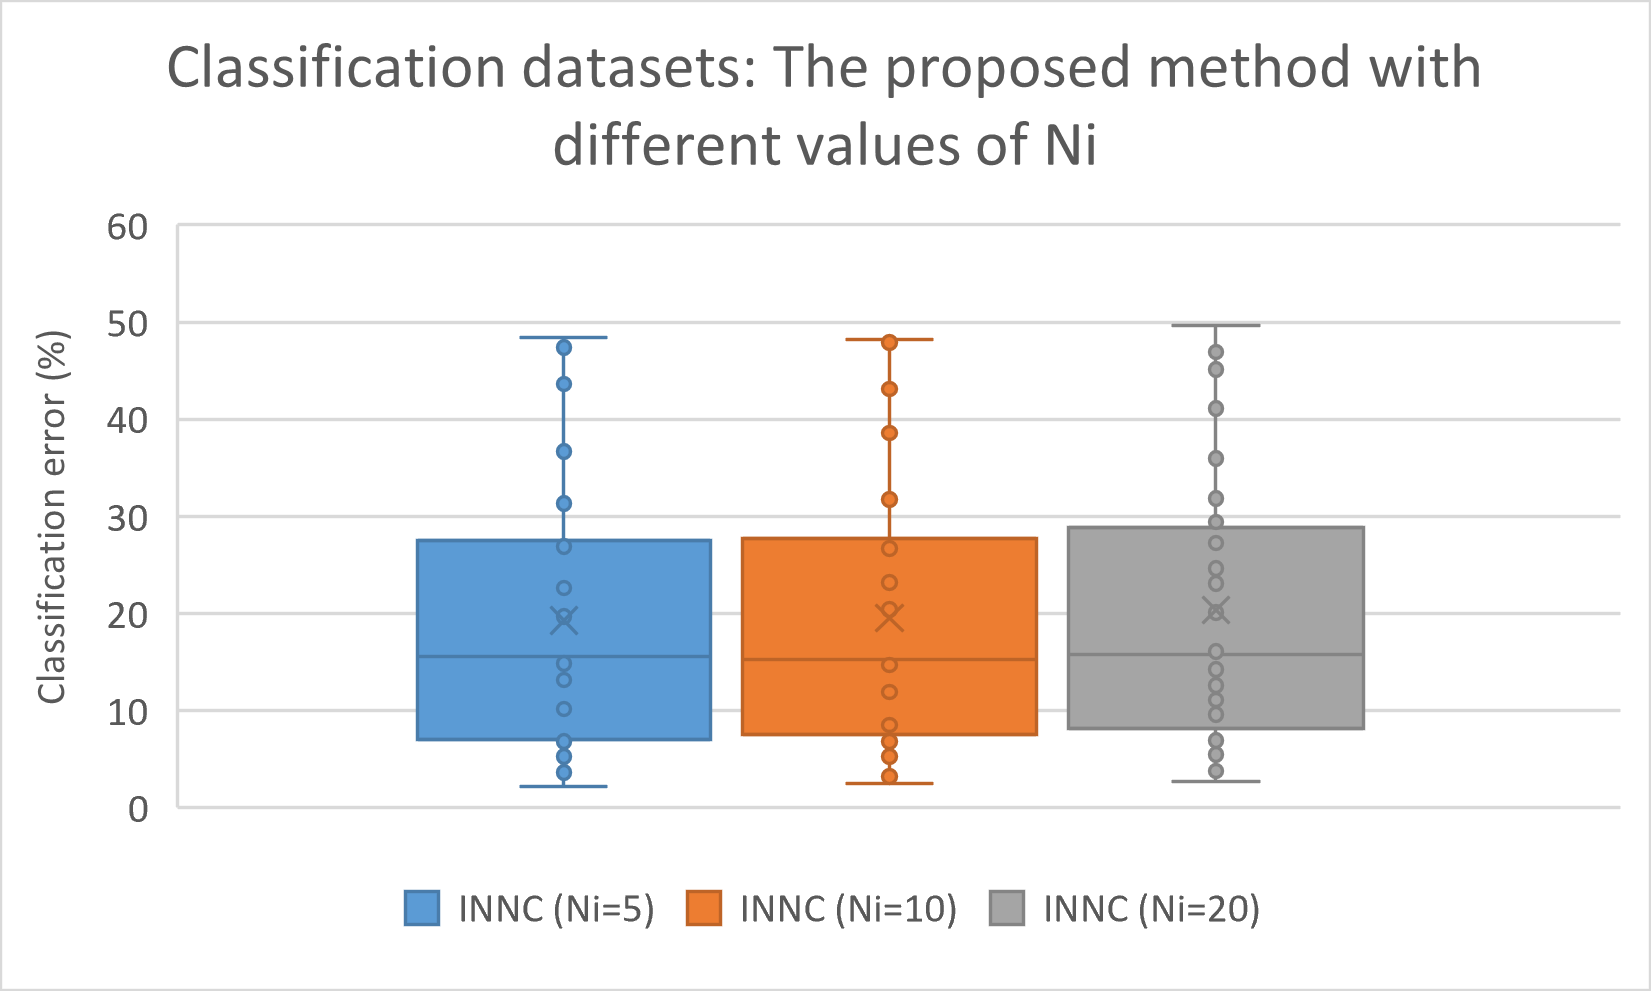
\includegraphics{table3}
\par\end{centering}
\caption{Box plot for the experiments with the parameter $N_{I}$ and the current
work. The method was applied on the classification datasets.\label{fig:boxNIClass}}

\end{figure}
\begin{figure}[H]
\begin{centering}
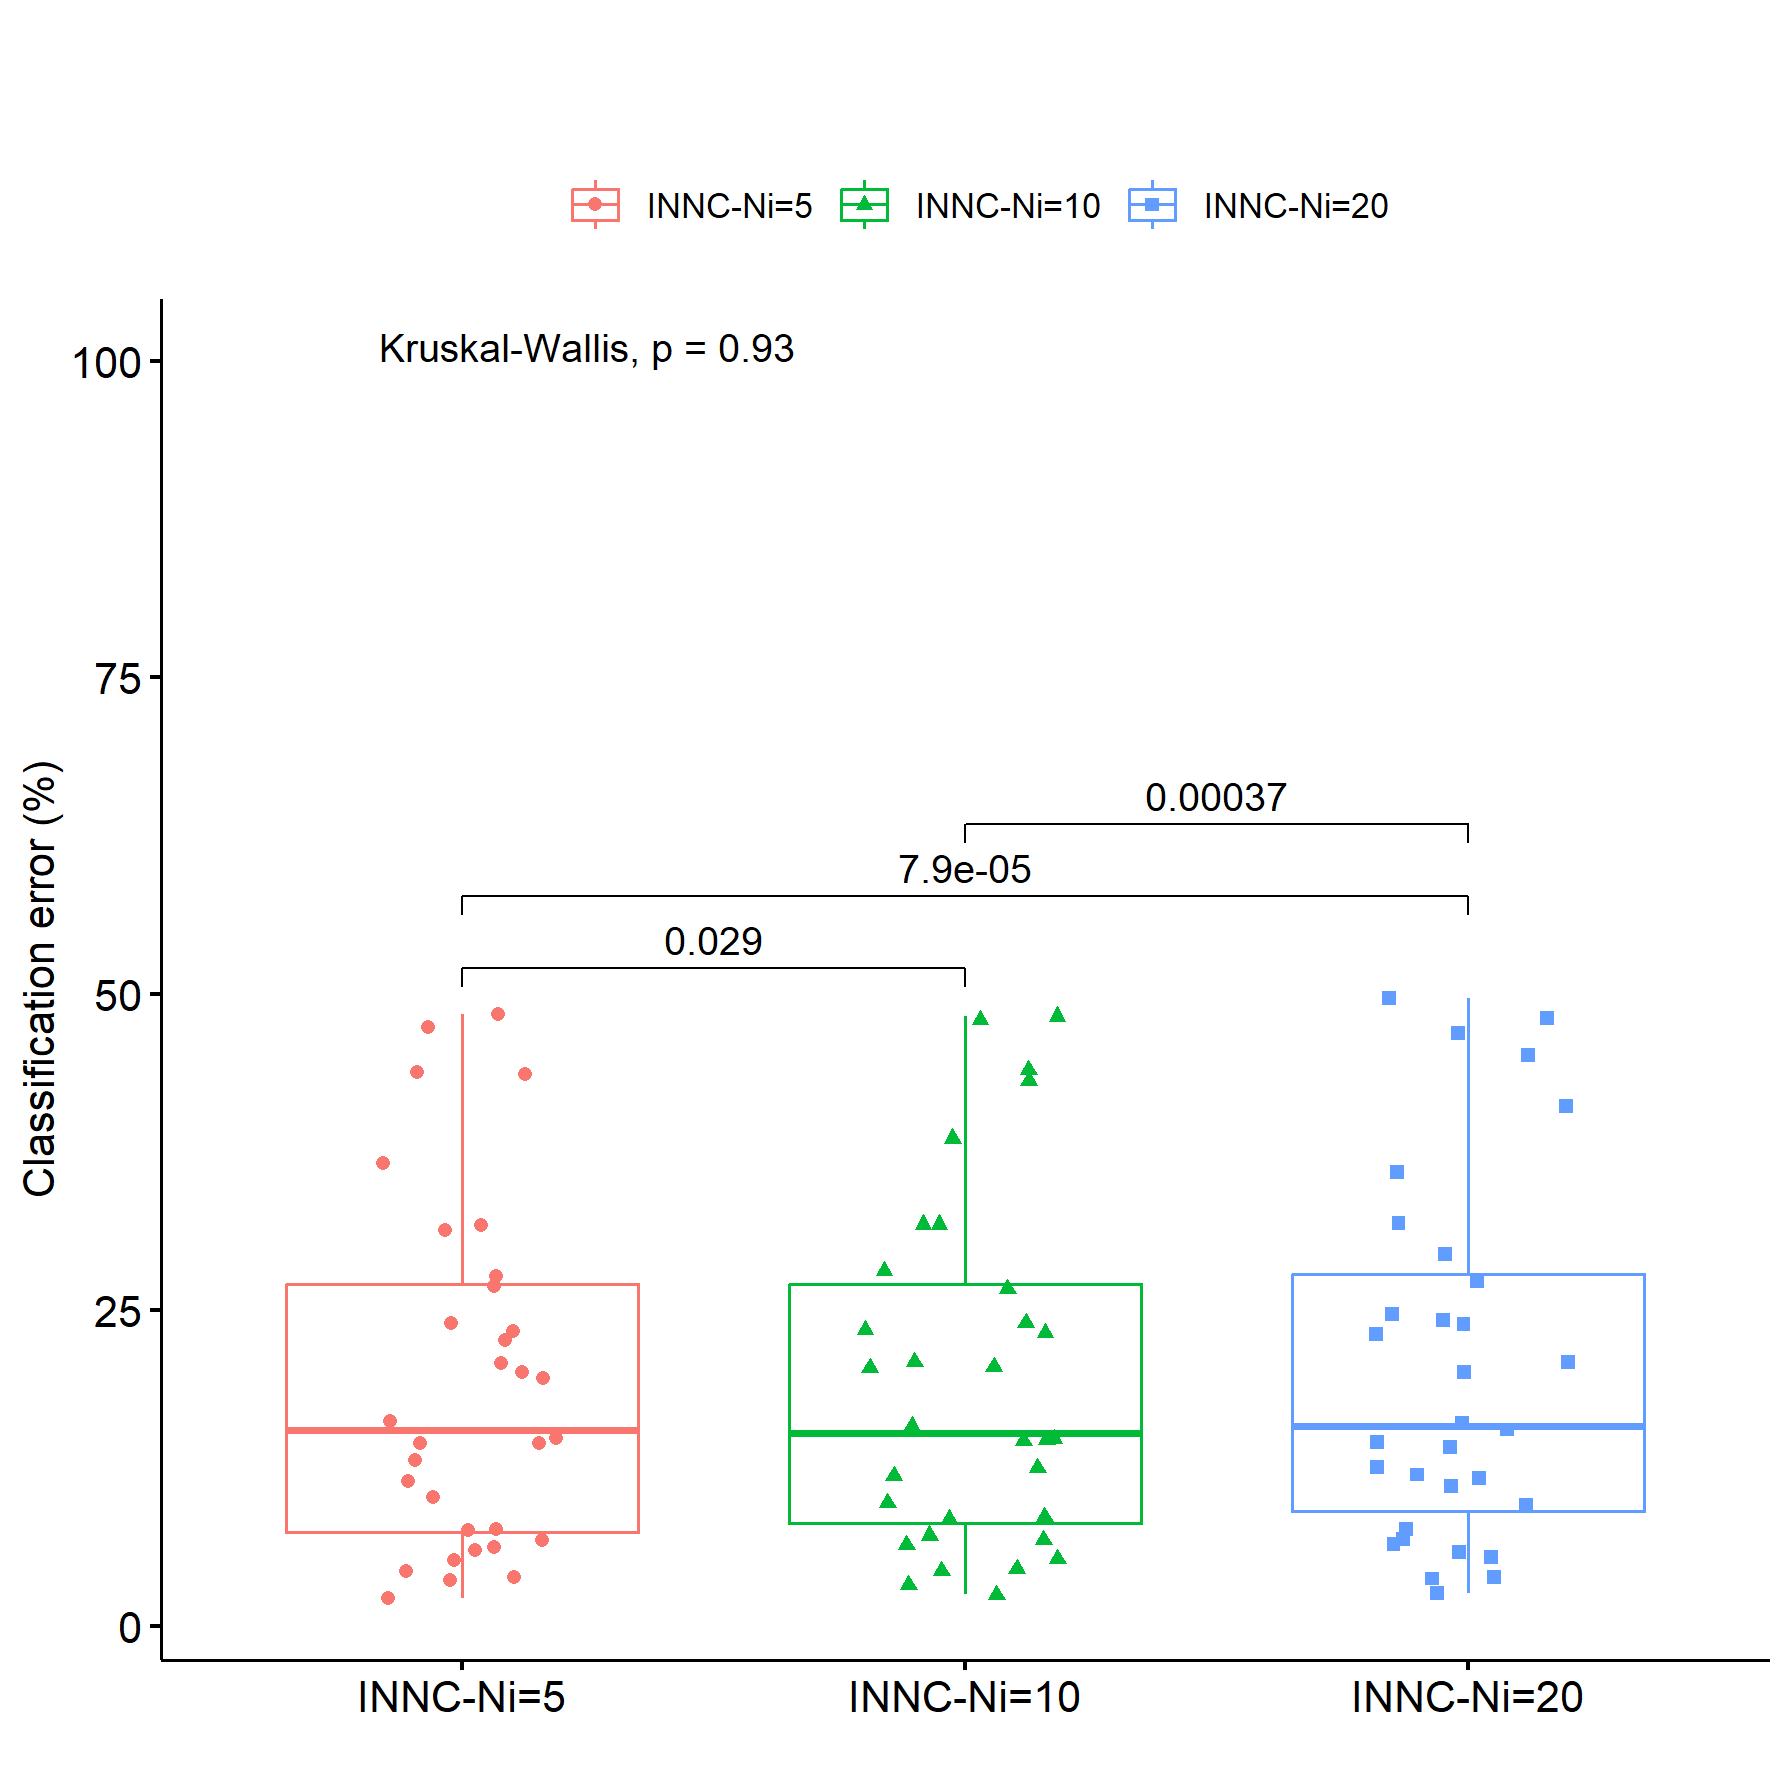
\includegraphics[scale=0.6]{table3_stat}
\par\end{centering}
\caption{Statistical comparison for the experiment with the current work and
a variety of values for parameter $N_{I}$. The method was applied
on the classification datasets.\label{fig:statNIClass}}

\end{figure}
In addition, the average execution time of the methods was recorded
for the various values of the parameter $N_{I}$ and the results are
shown in graphs \ref{fig:timeNIClass} and \ref{fig:timeNIRegression}
for classification and regression problems respectively.

\begin{figure}[H]
\begin{centering}
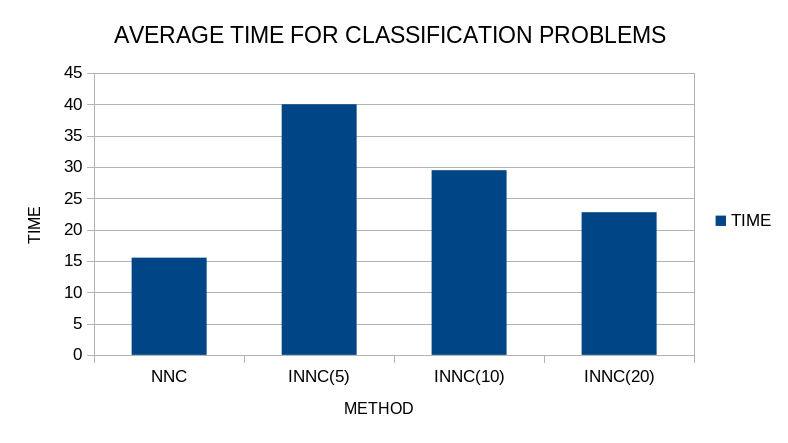
\includegraphics[scale=0.4]{innc_time_class}
\par\end{centering}
\caption{Average execution time for the original method and the modified one
for various values of the parameter $N_{I}.$ The experiments were
performed on the classification datasets.\label{fig:timeNIClass}}
\end{figure}
\begin{figure}[H]
\begin{centering}
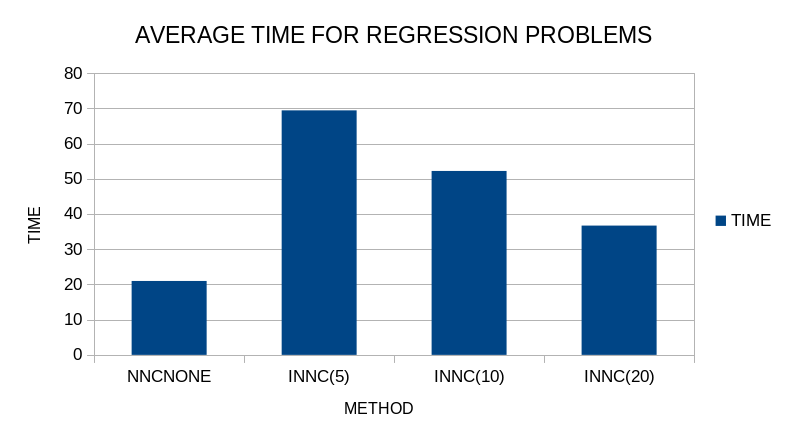
\includegraphics[scale=0.4]{innc_time_regression}
\par\end{centering}
\caption{Average execution time for the original method and the modified one
for various values of the parameter $N_{I}$. The execution times
were recorded for the regression problems.\label{fig:timeNIRegression}}

\end{figure}
As expected, the method requires more computational time than the
original one and in fact the smaller the value of the $N_{I}$ parameter
the more time has to be spent since more local optimizations have
to be performed. Of course, this additional computing time can be
significantly reduced by using parallel computing techniques.

\subsubsection{Experiments with the parameter $F$}

Another important parameter for the proposed method is the parameter
$F$. This parameter controls the range of changes that the local
optimization method can cause on randomly selected chromosomes. In
this experiment, the parameter $F$ changed from 1.5 to 8.0 and the
results for the classification datasets are outlined in Table \ref{tab:experFClass}
while the experimental results for the regression datasets are presented
in Table \ref{tab:experFRegression}.

\begin{table}[H]
\caption{Experimental results with a variety of values for the parameter $F$.
The method was applied on the classification datasets.\label{tab:experFClass}}

\centering{}%
\begin{tabular}{|c|c|c|c|c|}
\hline 
\textbf{DATASET} & \textbf{INNC$\left(F=1.5\right)$} & \textbf{INNC$\left(F=2.0\right)$} & \textbf{INNC$\left(F=4.0\right)$} & \textbf{INNC$\left(F=8.0\right)$}\tabularnewline
\hline 
\hline 
APPENDICITIS & 14.80\% & \textbf{14.20\%} & 14.70\% & 15.00\%\tabularnewline
\hline 
AUSTRALIAN & 14.58\% & 14.56\% & 14.80\% & \textbf{14.54\%}\tabularnewline
\hline 
BALANCE & \textbf{8.52\%} & 8.68\% & 8.66\% & 9.35\%\tabularnewline
\hline 
CIRCULAR & 5.92\% & 5.46\% & \textbf{5.32\%} & 5.43\%\tabularnewline
\hline 
CLEVELAND & 48.35\% & \textbf{47.38\%} & 47.93\% & 49.62\%\tabularnewline
\hline 
DERMATOLOGY & \textbf{19.80\%} & 20.09\% & 20.89\% & 21.66\%\tabularnewline
\hline 
ECOLI & \textbf{47.76\%} & 48.30\% & 48.21\% & 48.42\%\tabularnewline
\hline 
FERT & 21.20\% & 21.20\% & \textbf{20.50\%} & 20.90\%\tabularnewline
\hline 
HABERMAN & 26.43\% & \textbf{25.93\%} & 26.70\% & 26.70\%\tabularnewline
\hline 
HAYES-ROTH & 32.15\% & \textbf{31.31\%} & 31.77\% & 35.69\%\tabularnewline
\hline 
HEART & 14.81\% & 15.41\% & \textbf{14.74\%} & 15.41\%\tabularnewline
\hline 
HEARTATTACK & 21.20\% & \textbf{19.90\%} & 20.43\% & 20.40\%\tabularnewline
\hline 
HOUSEVOTES & 3.35\% & 3.65\% & \textbf{3.26\%} & 3.65\%\tabularnewline
\hline 
IONOSPHERE & 11.31\% & \textbf{10.40\%} & 11.92\% & 11.23\%\tabularnewline
\hline 
LIVERDISORDER & 32.09\% & \textbf{31.21\%} & 31.77\% & 33.18\%\tabularnewline
\hline 
MAMMOGRAPHIC & 16.15\% & 16.05\% & \textbf{15.81\%} & 16.07\%\tabularnewline
\hline 
PARKINSONS & 12.63\% & \textbf{12.47\%} & 12.53\% & 13.05\%\tabularnewline
\hline 
PIMA & \textbf{23.58\%} & 23.80\% & 24.00\% & 23.79\%\tabularnewline
\hline 
POPFAILURES & \textbf{5.85\%} & 6.29\% & 6.44\% & 6.04\%\tabularnewline
\hline 
REGIONS2 & 24.08\% & 23.48\% & \textbf{23.18\%} & 25.25\%\tabularnewline
\hline 
SAHEART & 28.41\% & 28.83\% & \textbf{28.09\%} & 28.30\%\tabularnewline
\hline 
SEGMENT & 45.12\% & 43.37\% & \textbf{43.12\%} & 43.93\%\tabularnewline
\hline 
SPIRAL & \textbf{43.40\%} & 43.72\% & 43.99\% & 44.61\%\tabularnewline
\hline 
STUDENT & 4.25\% & \textbf{4.15\%} & 4.55\% & 4.52\%\tabularnewline
\hline 
TRANSFUSION & 23.09\% & \textbf{22.93\%} & 23.43\% & 23.05\%\tabularnewline
\hline 
WDBC & 5.27\% & 5.30\% & \textbf{4.41\%} & 4.84\%\tabularnewline
\hline 
WINE & 10.53\% & 10.24\% & \textbf{9.77\%} & 11.59\%\tabularnewline
\hline 
Z\_F\_S & 9.20\% & \textbf{7.57\%} & 8.53\% & 8.63\%\tabularnewline
\hline 
Z\_O\_N\_F\_S & 40.60\% & 38.70\% & \textbf{38.58\%} & 39.78\%\tabularnewline
\hline 
ZO\_NF\_S & 6.90\% & 7.68\% & 6.84\% & \textbf{6.56\%}\tabularnewline
\hline 
ZONF\_S & 2.64\% & 2.72\% & \textbf{2.52\%} & 2.88\%\tabularnewline
\hline 
ZOO & 8.60\% & 7.40\% & \textbf{7.20\%} & 8.90\%\tabularnewline
\hline 
\textbf{AVERAGE} & \textbf{19.77\%} & \textbf{19.45\%} & \textbf{19.52\%} & \textbf{20.09\%}\tabularnewline
\hline 
\end{tabular}
\end{table}
\begin{table}[H]
\caption{Experimental results using a variety of values for the parameter $F$
. The method was applied on the regression datasets.\label{tab:experFRegression}}

\centering{}%
\begin{tabular}{|c|c|c|c|c|}
\hline 
\textbf{DATASET} & \textbf{INNC$\left(F=1.5\right)$} & \textbf{INNC$\left(F=2.0\right)$} & \textbf{INNC$\left(F=4.0\right)$} & \textbf{INNC$\left(F=8.0\right)$}\tabularnewline
\hline 
\hline 
ABALONE & 4.49 & 4.43 & \textbf{4.33} & 4.66\tabularnewline
\hline 
AIRFOIL & 0.002 & 0.002 & \textbf{0.002} & 0.002\tabularnewline
\hline 
BASEBALL & \textbf{48.31} & 50.38 & 48.42 & 48.52\tabularnewline
\hline 
BK & 0.06 & 0.21 & 0.07 & \textbf{0.02}\tabularnewline
\hline 
BL & 0.003 & 0.004 & \textbf{0.002} & 0.003\tabularnewline
\hline 
CONCRETE & \textbf{0.005} & 0.005 & 0.005 & 0.005\tabularnewline
\hline 
DEE & \textbf{0.23} & 0.23 & 0.23 & 0.23\tabularnewline
\hline 
HO & \textbf{0.01} & 0.01 & 0.01 & 0.01\tabularnewline
\hline 
HOUSING & 16.91 & 16.34 & \textbf{16.01} & 16.96\tabularnewline
\hline 
FY & 0.042 & 0.043 & \textbf{0.042} & 0.043\tabularnewline
\hline 
LASER & 0.005 & 0.005 & 0.005 & \textbf{0.004}\tabularnewline
\hline 
LW & \textbf{0.011} & 0.012 & 0.012 & 0.012\tabularnewline
\hline 
MORTGAGE & 0.027 & 0.025 & 0.026 & \textbf{0.024}\tabularnewline
\hline 
MUNDIAL & 0.035 & \textbf{0.033} & 0.034 & 0.23\tabularnewline
\hline 
PL & \textbf{0.022} & 0.022 & 0.022 & 0.022\tabularnewline
\hline 
QUAKE & \textbf{0.036} & 0.037 & 0.04 & 0.036\tabularnewline
\hline 
REALESTATE & 72.40 & 71.16 & 70.99 & \textbf{70.76}\tabularnewline
\hline 
SN & 0.024 & 0.024 & \textbf{0.023} & 0.024\tabularnewline
\hline 
TREASURY & 0.07 & 0.068 & \textbf{0.066} & 0.068\tabularnewline
\hline 
TZ & \textbf{0.029} & 0.031 & 0.03 & 0.031\tabularnewline
\hline 
VE & 0.032 & 0.03 & \textbf{0.025} & 0.028\tabularnewline
\hline 
\textbf{AVERAGE} & \textbf{6.80} & \textbf{6.81} & \textbf{6.69} & \textbf{6.75}\tabularnewline
\hline 
\end{tabular}
\end{table}
Once again, there are no significant differences in the performance
of the proposed technique as the critical factor $F$ varies. In the
case of the classification data, however, there is a small increase
in the classification error as this factor increases, which may be
due to the fact that, as we move away from the solution created by
the method of creating neural networks, the performance of the method
decreases. Also, the box plot for the classification datasets is depicted
in Figure \ref{fig:boxFClass}.

\begin{figure}[H]
\begin{centering}
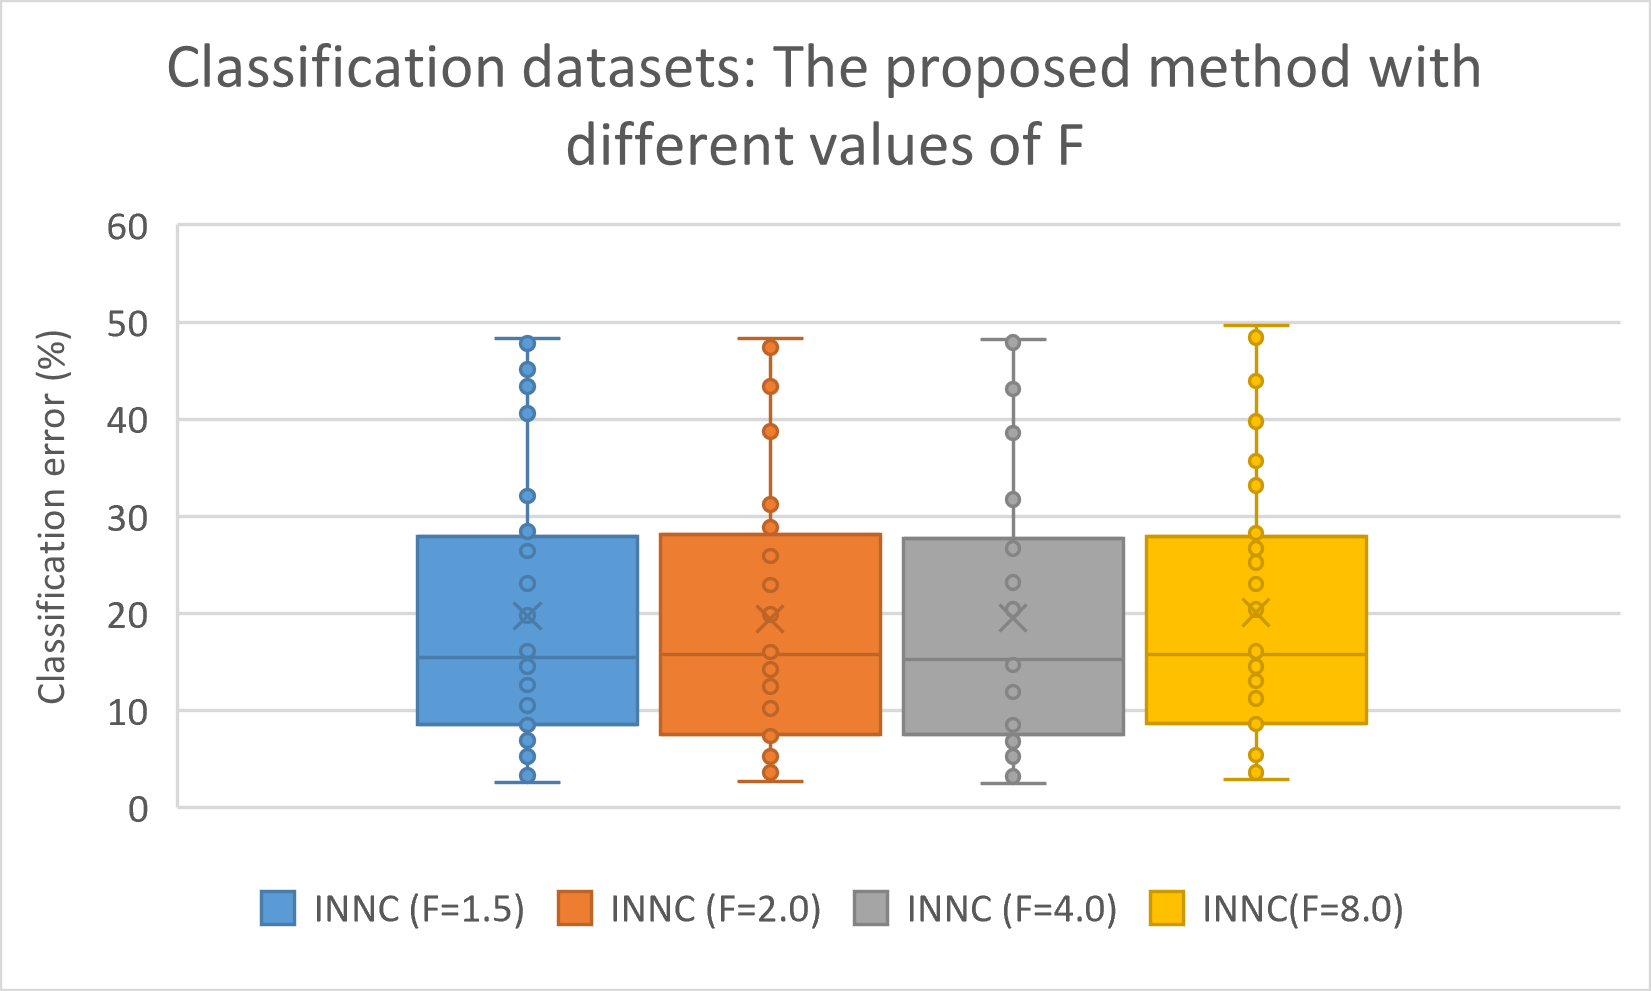
\includegraphics{table5}
\par\end{centering}
\caption{Box plot for the experiments using the current work and different
values of the parameter $F$. The method was applied on the classification
datasets.\label{fig:boxFClass}}

\end{figure}


\subsubsection{Experiments with the used local search optimizer}

An important issue of the proposed method is the selection of the
local search optimizer, that will be applied periodically to chromosomes
selected randomly. In the current work, a BFGS variant \citep{powell}
was chosen since it can satisfactorily handle the constraints placed
on the network parameters for the optimization. However, an additional
experiment was executed using different local optimization techniques
and the results for the classification datasets are presented in Table
\ref{tab:experLocalClass} and the results for the regression datasets
are shown in Table \ref{tab:experLocalRegression}. The following
notation is used in the experimental tables:
\begin{enumerate}
\item The column ADAM denotes the incorporation of the ADAM local optimization
method \citep{Adam} in the current technique.
\item The column LBFGS stands for the application of Limited Memory BFGS
(L-BFGS) method \citep{LBFGS} in used technique as the local search
procedure.
\item The column BFGS represents the incorporation of the BFGS method, modified
by Powell \citep{powell} as the local search procedure.
\end{enumerate}
\begin{table}[H]
\caption{Experimental results with different local optimization techniques
in the proposed method. The method was applied on the classification
datasets.\label{tab:experLocalClass}}

\centering{}%
\begin{tabular}{|c|c|c|c|}
\hline 
\textbf{DATASET} & \textbf{ADAM} & \textbf{LBFGS} & \textbf{BFGS}\tabularnewline
\hline 
\hline 
APPENDICITIS & \textbf{14.60\%} & 14.60\% & 14.70\%\tabularnewline
\hline 
AUSTRALIAN & \textbf{14.78\%} & 15.29\% & 14.80\%\tabularnewline
\hline 
BALANCE & 16.89\% & 11.47\% & \textbf{8.66\%}\tabularnewline
\hline 
CIRCULAR & 10.79\% & 8.15\% & \textbf{5.32\%}\tabularnewline
\hline 
CLEVELAND & 49.10\% & 48.45\% & \textbf{47.93\%}\tabularnewline
\hline 
DERMATOLOGY & 22.32\% & 23.03\% & \textbf{20.89\%}\tabularnewline
\hline 
ECOLI & \textbf{48.15\%} & 49.48\% & 48.21\%\tabularnewline
\hline 
FERT & \textbf{18.10\%} & 20.10\% & 20.50\%\tabularnewline
\hline 
HABERMAN & \textbf{26.27\%} & 26.63\% & 26.70\%\tabularnewline
\hline 
HAYES-ROTH & 36.23\% & 36.31\% & \textbf{31.77\%}\tabularnewline
\hline 
HEART & 15.71\% & 15.00\% & \textbf{14.74\%}\tabularnewline
\hline 
HEARTATTACK & 21.33\% & 20.07\% & 20.43\%\tabularnewline
\hline 
HOUSEVOTES & 3.39\% & 3.39\% & \textbf{3.26\%}\tabularnewline
\hline 
IONOSPHERE & \textbf{10.88\%} & 11.29\% & 11.92\%\tabularnewline
\hline 
LIVERDISORDER & 31.80\% & 33.18\% & \textbf{31.77\%}\tabularnewline
\hline 
MAMMOGRAPHIC & 16.71\% & 16.30\% & \textbf{15.81\%}\tabularnewline
\hline 
PARKINSONS & \textbf{12.10\%} & 12.32\% & 12.53\%\tabularnewline
\hline 
PIMA & 25.49\% & 24.97\% & \textbf{24.00\%}\tabularnewline
\hline 
POPFAILURES & \textbf{6.20\%} & 6.31\% & 6.44\%\tabularnewline
\hline 
REGIONS2 & 24.20\% & 24.06\% & \textbf{23.18\%}\tabularnewline
\hline 
SAHEART & 28.87\% & 28.96\% & \textbf{28.09\%}\tabularnewline
\hline 
SEGMENT & 50.16\% & 46.63\% & \textbf{43.12\%}\tabularnewline
\hline 
SPIRAL & 46.33\% & 45.24\% & 43.99\%\tabularnewline
\hline 
STUDENT & 4.05\% & \textbf{3.98\%} & 4.55\%\tabularnewline
\hline 
TRANSFUSION & 24.74\% & 24.56\% & \textbf{23.43\%}\tabularnewline
\hline 
WDBC & 6.30\% & 5.66\% & \textbf{4.41\%}\tabularnewline
\hline 
WINE & 11.47\% & 10.06\% & \textbf{9.77\%}\tabularnewline
\hline 
Z\_F\_S & 12.33\% & 10.92\% & \textbf{8.53\%}\tabularnewline
\hline 
Z\_O\_N\_F\_S & 41.40\% & 45.77\% & \textbf{38.58\%}\tabularnewline
\hline 
ZO\_NF\_S & 11.26\% & 9.83\% & \textbf{6.84\%}\tabularnewline
\hline 
ZONF\_S & 2.64\% & \textbf{2.35\%} & 2.52\%\tabularnewline
\hline 
ZOO & 8.50\% & 8.70\% & \textbf{7.20\%}\tabularnewline
\hline 
\textbf{AVERAGE} & \textbf{21.03\%} & \textbf{20.72\%} & \textbf{19.52\%}\tabularnewline
\hline 
\end{tabular}
\end{table}
\begin{table}[H]
\caption{Experimental results with local optimization techniques in the current
work. The method was applied on the regression datasets.\label{tab:experLocalRegression}}

\centering{}%
\begin{tabular}{|c|c|c|c|}
\hline 
\textbf{DATASET} & \textbf{ADAM} & \textbf{LBFGS} & \textbf{BFGS}\tabularnewline
\hline 
\hline 
ABALONE & 4.73 & 4.49 & \textbf{4.33}\tabularnewline
\hline 
AIRFOIL & 0.003 & 0.003 & \textbf{0.002}\tabularnewline
\hline 
BASEBALL & 53.98 & 51.88 & \textbf{48.42}\tabularnewline
\hline 
BK & \textbf{0.05} & 0.08 & 0.07\tabularnewline
\hline 
BL & 0.013 & 0.007 & \textbf{0.002}\tabularnewline
\hline 
CONCRETE & 0.006 & 0.006 & \textbf{0.005}\tabularnewline
\hline 
DEE & 0.24 & \textbf{0.23} & 0.23\tabularnewline
\hline 
HO & 0.012 & 0.012 & \textbf{0.01}\tabularnewline
\hline 
HOUSING & 20.20 & 20.49 & \textbf{16.01}\tabularnewline
\hline 
FY & \textbf{0.042} & 0.042 & 0.042\tabularnewline
\hline 
LASER & 0.012 & \textbf{0.005} & 0.005\tabularnewline
\hline 
LW & \textbf{0.011} & 0.011 & 0.012\tabularnewline
\hline 
MORTGAGE & 0.068 & 0.084 & \textbf{0.026}\tabularnewline
\hline 
MUNDIAL & 0.033 & \textbf{0.029} & 0.034\tabularnewline
\hline 
PL & 0.031 & 0.023 & \textbf{0.022}\tabularnewline
\hline 
QUAKE & \textbf{0.036} & 0.037 & 0.04\tabularnewline
\hline 
REALESTATE & 74.66 & 74.49 & \textbf{70.99}\tabularnewline
\hline 
SN & 0.025 & 0.024 & \textbf{0.023}\tabularnewline
\hline 
TREASURY & 0.114 & 0.084 & \textbf{0.066}\tabularnewline
\hline 
TZ & \textbf{0.03} & 0.08 & 0.03\tabularnewline
\hline 
VE & \textbf{0.024} & 0.132 & 0.025\tabularnewline
\hline 
\textbf{AVERAGE} & \textbf{7.35} & \textbf{7.25} & \textbf{6.69}\tabularnewline
\hline 
\end{tabular}
\end{table}
The BFGS method achieved lower values for the test error in the majority
of cases and this is also evident in the Figure \ref{fig:boxMethodClass},
where a box plot is depicted for the classification datasets.

\begin{figure}[H]
\begin{centering}
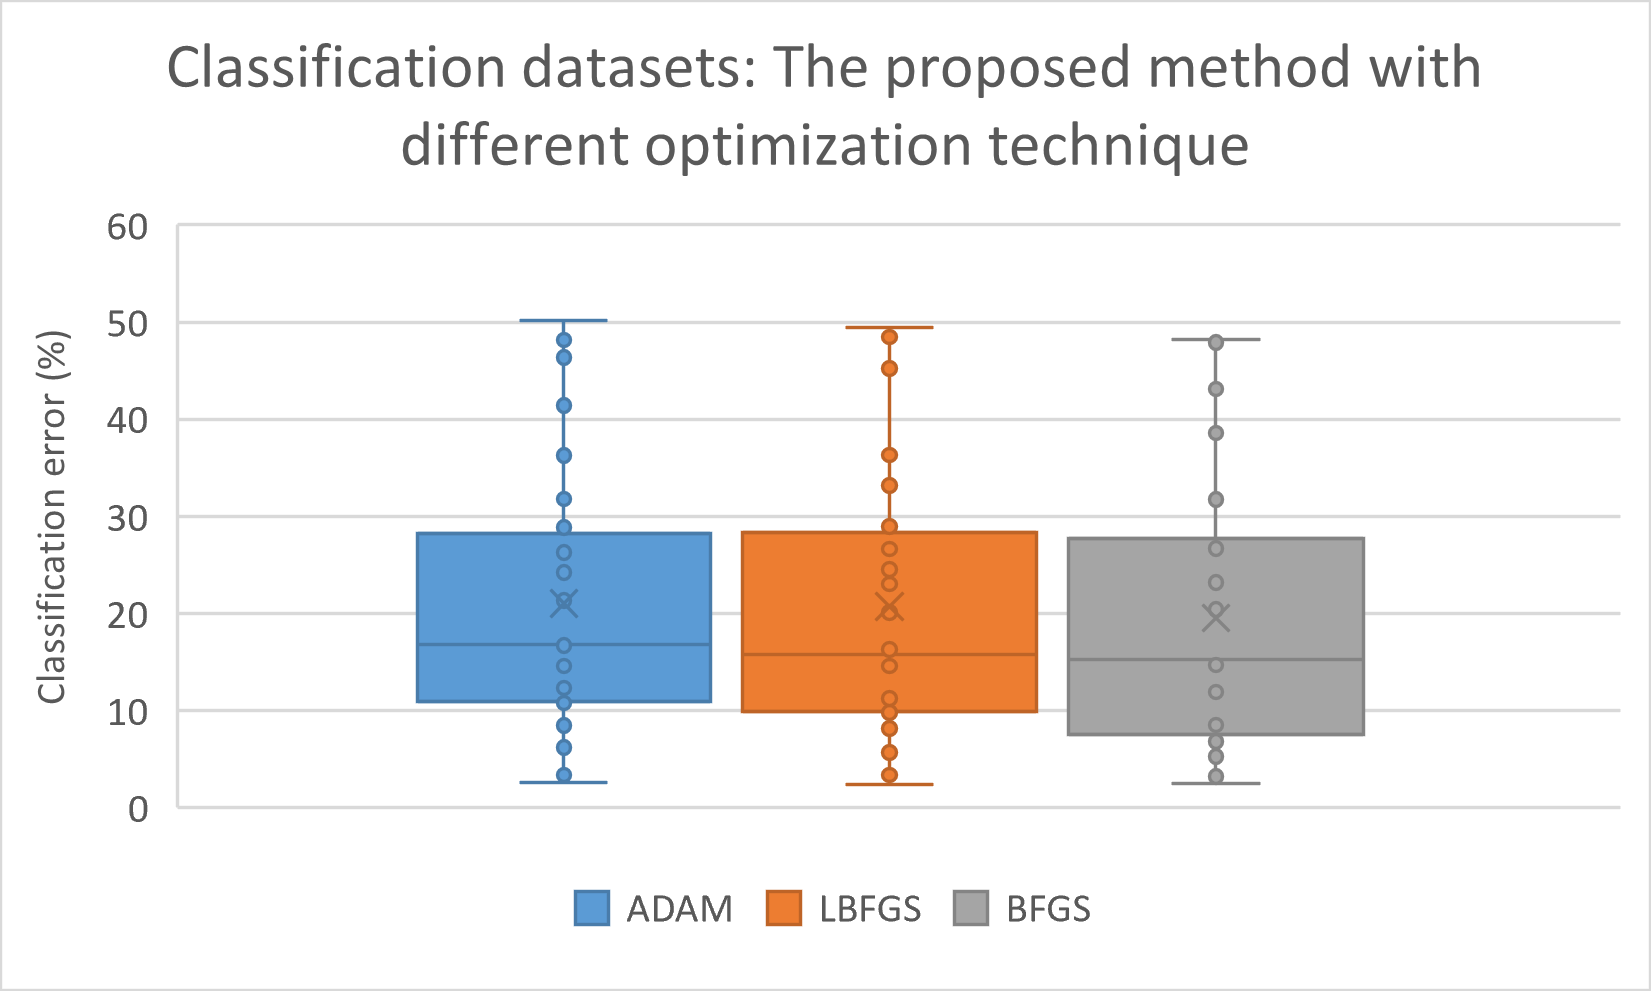
\includegraphics{table7}
\par\end{centering}
\caption{Box plot for the experiment with the proposed method and different
local optimization methods. The current work was executed on the classification
datasets.\label{fig:boxMethodClass}}

\end{figure}


\section{Conclusions\label{sec:Conclusions}}

An extension of the artificial neural network construction technique
was presented in the present work, in which the continuous application
of a local optimization method to chromosomes that selected randomly,
was introduced. The application of the local optimization method is
done in such a way as not to alter the architecture of the neural
network constructed by Grammatical Evolution. The proposed modified
method was applied on a series of benchmark datasets found in the
relevant literature and, judging from the experimental results, it
reduced significantly the test error of the original method in most
datasets. 

Moreover, to establish the stability of the proposed technique, a
series of experiments were executed in which a number of critical
parameters were varied over a range of values. After the completion
of these experiments, it became clear that there is no significant
difference in the effectiveness of the proposed method, even if these
critical parameters change significantly from execution to execution.
The only case where a significant difference in the effectiveness
of the proposed technique was found was when different local optimization
techniques were used, where the BFGS variant appeared to achieve the
best results in the majority of cases.

Nevertheless, one major drawback of the current work is the additional
execution time required from the execution of the local search optimization
techniques. Since the Grammatical Evolution procedure is a modified
genetic algorithm, the generated artificial neural networks are independent
of themselves, parallel programming techniques may be used in order
to increase the speed of the method, such as the usage of MPI  \citep{MPI}
or the OpenMP library \citep{OPENMP}.

\vspace{6pt}


\authorcontributions{V.C. and I.G.T. performed the mentioned experiments. I.G.T. wrote
the used software and D.T., A.T. and V.C. performed the statistical
analysis and prepared the manuscript. All authors have read and agreed
to the published version of the manuscript.}

\funding{This research received no external funding.}

\institutionalreview{Not applicable.}

\institutionalreview{Not applicable.}

\institutionalreview{Not applicable.}

\acknowledgments{This research has been financed by the European Union : Next Generation
EU through the Program Greece 2.0 National Recovery and Resilience
Plan , under the call RESEARCH -- CREATE -- INNOVATE, project name
“iCREW: Intelligent small craft simulator for advanced crew training
using Virtual Reality techniques\textquotedbl{} (project code:TAEDK-06195).}

\conflictsofinterest{The authors declare no conflicts of interest.}

\begin{adjustwidth}{-\extralength}{0cm}{}

\reftitle{References}
\begin{thebibliography}{99}
\bibitem{nn1}Abiodun, O. I., Jantan, A., Omolara, A. E., Dada, K.
V., Mohamed, N. A., \& Arshad, H. (2018). State-of-the-art in artificial
neural network applications: A survey. Heliyon, 4(11).

\bibitem{nn2}Suryadevara, S., \& Yanamala, A. K. Y. (2021). A Comprehensive
Overview of Artificial Neural Networks: Evolution, Architectures,
and Applications. Revista de Inteligencia Artificial en Medicina,
12(1), 51-76.

\bibitem{nnphysics1}P. Baldi, K. Cranmer, T. Faucett et al, Parameterized
neural networks for high-energy physics, Eur. Phys. J. C \textbf{76},
2016.

\bibitem{nnphysics2}Baldi, P., Cranmer, K., Faucett, T., Sadowski,
P., \& Whiteson, D. (2016). Parameterized neural networks for high-energy
physics. The European Physical Journal C, 76(5), 1-7.

\bibitem{nnphysics3}G. Carleo,M. Troyer, Solving the quantum many-body
problem with artificial neural networks, Science \textbf{355}, pp.
602-606, 2017.

\bibitem{nnde1}Khoo, Y., Lu, J., \& Ying, L. (2021). Solving parametric
PDE problems with artificial neural networks. European Journal of
Applied Mathematics, 32(3), 421-435.

\bibitem{nn_solar}A. Kumar Yadav, S.S. Chandel, Solar radiation prediction
using Artificial Neural Network techniques: A review, Renewable and
Sustainable Energy Reviews \textbf{33}, pp. 772-781, 2014.

\bibitem{nnagr2}A. Escamilla-García, G.M. Soto-Zarazúa, M. Toledano-Ayala,
E. Rivas-Araiza, A. Gastélum-Barrios, Abraham,Applications of Artificial
Neural Networks in Greenhouse Technology and Overview for Smart Agriculture
Development, Applied Sciences \textbf{10}, Article number 3835, 2020.

\bibitem{nnchem1}Lin Shen, Jingheng Wu, and Weitao Yang, Multiscale
Quantum Mechanics/Molecular Mechanics Simulations with Neural Networks,
Journal of Chemical Theory and Computation \textbf{12}, pp. 4934-4946,
2016.

\bibitem{nnchem3}Jennifer N. Wei, David Duvenaud, and Alán Aspuru-Guzik,
Neural Networks for the Prediction of Organic Chemistry Reactions,
ACS Central Science \textbf{2}, pp. 725-732, 2016.

\bibitem{nn_wind}Khosravi, A. K. R. M. L. P. J., Koury, R. N. N.,
Machado, L., \& Pabon, J. J. G. (2018). Prediction of wind speed and
wind direction using artificial neural network, support vector regression
and adaptive neuro-fuzzy inference system. Sustainable Energy Technologies
and Assessments, 25, 146-160.

\bibitem{nnecon1}Lukas Falat and Lucia Pancikova, Quantitative Modelling
in Economics with Advanced Artificial Neural Networks, Procedia Economics
and Finance \textbf{34}, pp. 194-201, 2015.

\bibitem{nnecon2}Mohammad Namazi, Ahmad Shokrolahi, Mohammad Sadeghzadeh
Maharluie, Detecting and ranking cash flow risk factors via artificial
neural networks technique, Journal of Business Research \textbf{69},
pp. 1801-1806, 2016.

\bibitem{nnmed1}Igor I. Baskin, David Winkler and Igor V. Tetko,
A renaissance of neural networks in drug discovery, Expert Opinion
on Drug Discovery \textbf{11}, pp. 785-795, 2016.

\bibitem{nnmed2}Ronadl Bartzatt, Prediction of Novel Anti-Ebola Virus
Compounds Utilizing Artificial Neural Network (ANN), Chemistry Faculty
Publications \textbf{49}, pp. 16-34, 2018.

\bibitem{bpnn1}Vora, K., \& Yagnik, S. (2014). A survey on backpropagation
algorithms for feedforward neural networks. International Journal
of Engineering Development and Research, 1(3), 193-197.

\bibitem{bpnn2}K. Vora, S. Yagnik, A survey on backpropagation algorithms
for feedforward neural networks, International Journal of Engineering
Development and Research \textbf{1}, pp. 193-197, 2014.

\bibitem{rpropnn-1}Pajchrowski, T., Zawirski, K., \& Nowopolski,
K. (2014). Neural speed controller trained online by means of modified
RPROP algorithm. IEEE transactions on industrial informatics, 11(2),
560-568.

\bibitem{rpropnn-2}Hermanto, R. P. S., \& Nugroho, A. (2018). Waiting-time
estimation in bank customer queues using RPROP neural networks. Procedia
Computer Science, 135, 35-42.

\bibitem{nn_adam}D. P. Kingma, J. L. Ba, ADAM: a method for stochastic
optimization, in: Proceedings of the 3rd International Conference
on Learning Representations (ICLR 2015), pp. 1--15, 2015.

\bibitem{nn_siman2}C.L. Kuo, E.E. Kuruoglu, W.K.V. Chan, Neural Network
Structure Optimization by Simulated Annealing, Entropy \textbf{24},
348, 2022.

\bibitem{geneticnn1}Reynolds, J., Rezgui, Y., Kwan, A., \& Piriou,
S. (2018). A zone-level, building energy optimisation combining an
artificial neural network, a genetic algorithm, and model predictive
control. Energy, 151, 729-739.

\bibitem{psonn}Das, G., Pattnaik, P. K., \& Padhy, S. K. (2014).
Artificial neural network trained by particle swarm optimization for
non-linear channel equalization. Expert Systems with Applications,
41(7), 3491-3496.

\bibitem{weight_de1}Wang, L., Zeng, Y., \& Chen, T. (2015). Back
propagation neural network with adaptive differential evolution algorithm
for time series forecasting. Expert Systems with Applications, 42(2),
855-863.

\bibitem{weight_aco}K.M. Salama, A.M. Abdelbar, Learning neural network
structures with ant colony algorithms, Swarm Intell \textbf{9}, pp.
229--265, 2015.

\bibitem{gwo_nn}S. Mirjalili, How effective is the Grey Wolf optimizer
in training multi-layer perceptrons, Appl Intell \textbf{43}, pp.
150--161, 2015.

\bibitem{whale_nn}I. Aljarah, H. Faris, S. Mirjalili, Optimizing
connection weights in neural networks using the whale optimization
algorithm, Soft Comput \textbf{22}, pp. 1--15, 2018. 

\bibitem{nn_gpu3}M. Zhang, K. Hibi, J. Inoue, GPU-accelerated artificial
neural network potential for molecular dynamics simulation, Computer
Physics Communications \textbf{285}, 108655, 2023.

\bibitem{nn_init1}T.M. Varnava, A.J.Meade, An initialization method
for feedforward artificial neural networks using polynomial bases,
Advances in Adaptive Data Analysis \textbf{3}, pp. 385-400, 2011.

\bibitem{nn_init2}I. Ivanova, M. Kubat, Initialization of neural
networks by means of decision trees, Knowledge-Based Systems \textbf{8},
pp. 333-344, 1995.

\bibitem{nn_init3}S.S. Sodhi, P. Chandra, Interval based Weight Initialization
Method for Sigmoidal Feedforward Artificial Neural Networks, AASRI
Procedia \textbf{6}, pp. 19-25, 2014.

\bibitem{nn_init4}K. Chumachenko, A. Iosifidis, M. Gabbouj, Feedforward
neural networks initialization based on discriminant learning, Neural
Networks \textbf{146}, pp. 220-229, 2022.

\bibitem{nn_init5}Q. Chen, W. Hao, J. He, A weight initialization
based on the linear product structure for neural networks, Applied
Mathematics and Computation \textbf{415}, 126722, 2022.

\bibitem{nn_arch1}J. Arifovic, R. Gençay, Using genetic algorithms
to select architecture of a feedforward artificial neural network,
Physica A: Statistical Mechanics and its Applications \textbf{289},
pp. 574-594, 2001.

\bibitem{nn_arch2}P.G. Benardos, G.C. Vosniakos, Optimizing feedforward
artificial neural network architecture, Engineering Applications of
Artificial Intelligence \textbf{20}, pp. 365-382, 2007.

\bibitem{nn_arch3}B.A. Garro, R.A. Vázquez, Designing Artificial
Neural Networks Using Particle Swarm Optimization Algorithms, Computational
Intelligence and Neuroscience, 369298, 2015. 

\bibitem{nn_arch4}B. Baker, O. Gupta, N. Naik, R. Raskar, Designing
neural network architectures using reinforcement learning. arXiv preprint
arXiv:1611.02167, 2016.

\bibitem{nn_arch5}M. M. Islam, M. A. Sattar, M. F. Amin, X. Yao,
K. Murase, A New Adaptive Merging and Growing Algorithm for Designing
Artificial Neural Networks, IEEE Transactions on Systems, Man, and
Cybernetics, Part B (Cybernetics) \textbf{39}, pp. 705-722, 2009. 

\bibitem{ge1}M. O’Neill, C. Ryan, Grammatical evolution, IEEE Trans.
Evol. Comput. \textbf{5,}pp. 349--358, 2001.

\bibitem{nnc}I.G. Tsoulos, D. Gavrilis, E. Glavas, Neural network
construction and training using grammatical evolution, Neurocomputing
\textbf{72}, pp. 269-277, 2008.

\bibitem{nnc_amide1}G.V. Papamokos, I.G. Tsoulos, I.N. Demetropoulos,
E. Glavas, Location of amide I mode of vibration in computed data
utilizing constructed neural networks, Expert Systems with Applications
\textbf{36}, pp. 12210-12213, 2009.

\bibitem{nnc_de}I.G. Tsoulos, D. Gavrilis, E. Glavas, Solving differential
equations with constructed neural networks, Neurocomputing \textbf{72},
pp. 2385-2391, 2009.

\bibitem{nnc_feas}I.G. Tsoulos, G. Mitsi, A. Stavrakoudis, S. Papapetropoulos,
Application of Machine Learning in a Parkinson's Disease Digital Biomarker
Dataset Using Neural Network Construction (NNC) Methodology Discriminates
Patient Motor Status, Frontiers in ICT 6, 10, 2019.

\bibitem{nnc_student}V. Christou, I.G. Tsoulos, V. Loupas, A.T. Tzallas,
C. Gogos, P.S. Karvelis, N. Antoniadis, E. Glavas, N. Giannakeas,
Performance and early drop prediction for higher education students
using machine learning, Expert Systems with Applications \textbf{225},
120079, 2023.

\bibitem{nnc_autism}E.I. Toki, J. Pange, G. Tatsis, K. Plachouras,
I.G. Tsoulos, Utilizing Constructed Neural Networks for Autism Screening,
Applied Sciences \textbf{14}, 3053, 2024.

\bibitem{nnc_code}I.G. Tsoulos, A.Tzallas, D. Tsalikakis, NNC: A
tool based on Grammatical Evolution for data classification and differential
equation solving, SoftwareX \textbf{10}, 100297, 2019.

\bibitem{bnf1}J. W. Backus. The Syntax and Semantics of the Proposed
International Algebraic Language of the Zurich ACM-GAMM Conference.
Proceedings of the International Conference on Information Processing,
UNESCO, 1959, pp.125-132.

\bibitem{ge_program1}C. Ryan, J. Collins, M. O’Neill, Grammatical
evolution: Evolving programs for an arbitrary language. In: Banzhaf,
W., Poli, R., Schoenauer, M., Fogarty, T.C. (eds) Genetic Programming.
EuroGP 1998. Lecture Notes in Computer Science, vol 1391. Springer,
Berlin, Heidelberg, 1998.

\bibitem{ge_program2}M. O’Neill, M., C. Ryan, Evolving Multi-line
Compilable C Programs. In: Poli, R., Nordin, P., Langdon, W.B., Fogarty,
T.C. (eds) Genetic Programming. EuroGP 1999. Lecture Notes in Computer
Science, vol 1598. Springer, Berlin, Heidelberg, 1999.

\bibitem{ge_trig}C. Ryan, M. O’Neill, J.J. Collins, Grammatical evolution:
Solving trigonometric identities, proceedings of Mendel. Vol. 98.
1998.

\bibitem{ge_music}A.O. Puente, R. S. Alfonso, M. A. Moreno, Automatic
composition of music by means of grammatical evolution, In: APL '02:
Proceedings of the 2002 conference on APL: array processing languages:
lore, problems, and applications July 2002 Pages 148--155. 

\bibitem{ge_constant}I. Dempsey, M.O' Neill, A. Brabazon, Constant
creation in grammatical evolution, International Journal of Innovative
Computing and Applications \textbf{1} , pp 23--38, 2007.

\bibitem{ge_pacman}E. Galván-López, J.M. Swafford, M. O’Neill, A.
Brabazon, Evolving a Ms. PacMan Controller Using Grammatical Evolution.
In: , et al. Applications of Evolutionary Computation. EvoApplications
2010. Lecture Notes in Computer Science, vol 6024. Springer, Berlin,
Heidelberg, 2010.

\bibitem{ge_supermario}N. Shaker, M. Nicolau, G. N. Yannakakis, J.
Togelius, M. O'Neill, Evolving levels for Super Mario Bros using grammatical
evolution, 2012 IEEE Conference on Computational Intelligence and
Games (CIG), 2012, pp. 304-31.

\bibitem{ge_energy}D. Martínez-Rodríguez, J. M. Colmenar, J. I. Hidalgo,
R.J. Villanueva Micó, S. Salcedo-Sanz, Particle swarm grammatical
evolution for energy demand estimation, Energy Science and Engineering
\textbf{8}, pp. 1068-1079, 2020.

\bibitem{ge_comb}N. R. Sabar, M. Ayob, G. Kendall, R. Qu, Grammatical
Evolution Hyper-Heuristic for Combinatorial Optimization Problems,
IEEE Transactions on Evolutionary Computation \textbf{17}, pp. 840-861,
2013.

\bibitem{ge_crypt}C. Ryan, M. Kshirsagar, G. Vaidya, G. et al. Design
of a cryptographically secure pseudo random number generator with
grammatical evolution. Sci Rep \textbf{12}, 8602, 2022.

\bibitem{ge_decision}P.J. Pereira, P. Cortez, R. Mendes, Multi-objective
Grammatical Evolution of Decision Trees for Mobile Marketing user
conversion prediction, Expert Systems with Applications \textbf{168},
114287, 2021.

\bibitem{ge_analog}F. Castejón, E.J. Carmona, Automatic design of
analog electronic circuits using grammatical evolution, Applied Soft
Computing \textbf{62}, pp. 1003-1018, 2018.

\bibitem{ge_wikipedia}L. Araujo, J. Martinez-Romo, A. Duque, Discovering
taxonomies in Wikipedia by means of grammatical evolution. Soft Comput
\textbf{22}, pp. 2907--2919, 2018. 

\bibitem{ge_trading}C. Martín, D. Quintana, P. Isasi, Grammatical
Evolution-based ensembles for algorithmic trading, Applied Soft Computing
\textbf{84}, 105713, 2019.

\bibitem{ge_bio}Moore, J.H., Sipper, M. (2018). Grammatical Evolution
Strategies for Bioinformatics and Systems Genomics. In: Ryan, C.,
O'Neill, M., Collins, J. (eds) Handbook of Grammatical Evolution.
Springer, Cham. https://doi.org/10.1007/978-3-319-78717-6\_16

\bibitem{ge_robotics}Peabody, C., \& Seitzer, J. (2015, March). GEF:
a self-programming robot using grammatical evolution. In Proceedings
of the AAAI Conference on Artificial Intelligence (Vol. 29, No. 1).

\bibitem{Hornik}Hornik, K., Stinchcombe, M., \& White, H. (1989).
Multilayer feedforward networks are universal approximators. Neural
networks, 2(5), 359-366.

\bibitem{powell}M.J.D Powell, A Tolerant Algorithm for Linearly Constrained
Optimization Calculations, Mathematical Programming \textbf{45}, pp.
547-566, 1989. 

\bibitem{UCL}M. Kelly, R. Longjohn, K. Nottingham, The UCI Machine
Learning Repository. 2023. Available online: https://archive.ics.uci.edu
(accessed on 18 February 2024).

\bibitem{Keel}J. Alcalá-Fdez, A. Fernandez, J. Luengo, J. Derrac,
S. García, L. Sánchez, F. Herrera. KEEL Data-Mining Software Tool:
Data Set Repository, Integration of Algorithms and Experimental Analysis
Framework. Journal of Multiple-Valued Logic and Soft Computing 17,
pp. 255-287, 2011.

\bibitem{appendicitis}Weiss, Sholom M. and Kulikowski, Casimir A.,
Computer Systems That Learn: Classification and Prediction Methods
from Statistics, Neural Nets, Machine Learning, and Expert Systems,
Morgan Kaufmann Publishers Inc, 1991.

\bibitem{australian}J.R. Quinlan, Simplifying Decision Trees. International
Journal of Man-Machine Studies \textbf{27}, pp. 221-234, 1987. 

\bibitem{balance}T. Shultz, D. Mareschal, W. Schmidt, Modeling Cognitive
Development on Balance Scale Phenomena, Machine Learning \textbf{16},
pp. 59-88, 1994.

\bibitem{cleveland1}Z.H. Zhou,Y. Jiang, NeC4.5: neural ensemble based
C4.5,\textquotedbl{} in IEEE Transactions on Knowledge and Data Engineering
\textbf{16}, pp. 770-773, 2004.

\bibitem{cleveland2}R. Setiono , W.K. Leow, FERNN: An Algorithm for
Fast Extraction of Rules from Neural Networks, Applied Intelligence
\textbf{12}, pp. 15-25, 2000.

\bibitem{dermatology}G. Demiroz, H.A. Govenir, N. Ilter, Learning
Differential Diagnosis of Eryhemato-Squamous Diseases using Voting
Feature Intervals, Artificial Intelligence in Medicine. \textbf{13},
pp. 147--165, 1998.

\bibitem{ecoli}P. Horton, K.Nakai, A Probabilistic Classification
System for Predicting the Cellular Localization Sites of Proteins,
In: Proceedings of International Conference on Intelligent Systems
for Molecular Biology \textbf{4}, pp. 109-15, 1996.

\bibitem{hayesroth}B. Hayes-Roth, B., F. Hayes-Roth. Concept learning
and the recognition and classification of exemplars. Journal of Verbal
Learning and Verbal Behavior \textbf{16}, pp. 321-338, 1977.

\bibitem{heart}I. Kononenko, E. Šimec, M. Robnik-Šikonja, Overcoming
the Myopia of Inductive Learning Algorithms with RELIEFF, Applied
Intelligence \textbf{7}, pp. 39--55, 1997

\bibitem{housevotes}R.M. French, N. Chater, Using noise to compute
error surfaces in connectionist networks: a novel means of reducing
catastrophic forgetting, Neural Comput. \textbf{14}, pp. 1755-1769,
2002.

\bibitem{liver} J. Garcke, M. Griebel, Classification with sparse
grids using simplicial basis functions, Intell. Data Anal. \textbf{6},
pp. 483-502, 2002.

\bibitem{ion1}J.G. Dy , C.E. Brodley, Feature Selection for Unsupervised
Learning, The Journal of Machine Learning Research \textbf{5}, pp
845--889, 2004.

\bibitem{ion2}S. J. Perantonis, V. Virvilis, Input Feature Extraction
for Multilayered Perceptrons Using Supervised Principal Component
Analysis, Neural Processing Letters \textbf{10}, pp 243--252, 1999.

\bibitem{mammographic}M. Elter, R. Schulz-Wendtland, T. Wittenberg,
The prediction of breast cancer biopsy outcomes using two CAD approaches
that both emphasize an intelligible decision process, Med Phys. \textbf{34},
pp. 4164-72, 2007.

\bibitem{parkinsons}M.A. Little, P.E. McSharry, E.J. Hunter, J. Spielman,
L.O. Ramig, Suitability of dysphonia measurements for telemonitoring
of Parkinson's disease. IEEE Trans Biomed Eng. \textbf{56}, pp. 1015-1022,
2009.

\bibitem{pima}J.W. Smith, J.E. Everhart, W.C. Dickson, W.C. Knowler,
R.S. Johannes, Using the ADAP learning algorithm to forecast the onset
of diabetes mellitus, In: Proceedings of the Symposium on Computer
Applications and Medical Care IEEE Computer Society Press, pp.261-265,
1988.

\bibitem{popfailures}D.D. Lucas, R. Klein, J. Tannahill, D. Ivanova,
S. Brandon, D. Domyancic, Y. Zhang, Failure analysis of parameter-induced
simulation crashes in climate models, Geoscientific Model Development
\textbf{6}, pp. 1157-1171, 2013.

\bibitem{regions}N. Giannakeas, M.G. Tsipouras, A.T. Tzallas, K.
Kyriakidi, Z.E. Tsianou, P. Manousou, A. Hall, E.C. Karvounis, V.
Tsianos, E. Tsianos, A clustering based method for collagen proportional
area extraction in liver biopsy images (2015) Proceedings of the Annual
International Conference of the IEEE Engineering in Medicine and Biology
Society, EMBS, 2015-November, art. no. 7319047, pp. 3097-3100. 

\bibitem{saheart}T. Hastie, R. Tibshirani, Non-parametric logistic
and proportional odds regression, JRSS-C (Applied Statistics) \textbf{36},
pp. 260--276, 1987.

\bibitem{segment}M. Dash, H. Liu, P. Scheuermann, K. L. Tan, Fast
hierarchical clustering and its validation, Data \& Knowledge Engineering
\textbf{44}, pp 109--138, 2003.

\bibitem{student}P. Cortez, A. M. Gonçalves Silva, Using data mining
to predict secondary school student performance, In Proceedings of
5th FUture BUsiness TEChnology Conference (FUBUTEC 2008) (pp. 5--12).
EUROSIS-ETI, 2008.

\bibitem{transfusion}I-Cheng Yeh, King-Jang Yang, Tao-Ming Ting,
Knowledge discovery on RFM model using Bernoulli sequence, Expert
Systems with Applications \textbf{36}, pp. 5866-5871, 2009.

\bibitem{wdbc}W.H. Wolberg, O.L. Mangasarian, Multisurface method
of pattern separation for medical diagnosis applied to breast cytology,
Proc Natl Acad Sci U S A. \textbf{87}, pp. 9193--9196, 1990.

\bibitem{wine1}M. Raymer, T.E. Doom, L.A. Kuhn, W.F. Punch, Knowledge
discovery in medical and biological datasets using a hybrid Bayes
classifier/evolutionary algorithm. IEEE transactions on systems, man,
and cybernetics. Part B, Cybernetics : a publication of the IEEE Systems,
Man, and Cybernetics Society, \textbf{33} , pp. 802-813, 2003.

\bibitem{wine2}P. Zhong, M. Fukushima, Regularized nonsmooth Newton
method for multi-class support vector machines, Optimization Methods
and Software \textbf{22}, pp. 225-236, 2007.

\bibitem{eeg}R.G. Andrzejak, K. Lehnertz, F. Mormann, C. Rieke, P.
David, and C. E. Elger, Indications of nonlinear deterministic and
finite-dimensional structures in time series of brain electrical activity:
Dependence on recording region and brain state, Phys. Rev. E \textbf{64},
pp. 1-8, 2001.

\bibitem{zoo}M. Koivisto, K. Sood, Exact Bayesian Structure Discovery
in Bayesian Networks, The Journal of Machine Learning Research\textbf{
5}, pp. 549--573, 2004.

\bibitem{abalone}Nash, W.J.; Sellers, T.L.; Talbot, S.R.; Cawthor,
A.J.; Ford, W.B. The Population Biology of Abalone (\_Haliotis\_ species)
in Tasmania. I. Blacklip Abalone (\_H. rubra\_) from the North Coast
and Islands of Bass Strait; Sea Fisheries Division, Technical Report
48; Sea Fisheries Division, Department of Primary Industry and Fisheries:
Orange, NSW, Australia, 1994.

\bibitem{airfoil}T.F. Brooks, D.S. Pope, A.M. Marcolini, Airfoil
self-noise and prediction. Technical report, NASA RP-1218, July 1989. 

\bibitem{Stat}J.S. Simonoff, Smooting Methods in Statistics, Springer
- Verlag, 1996.

\bibitem{concrete}I.Cheng Yeh, Modeling of strength of high performance
concrete using artificial neural networks, Cement and Concrete Research.
\textbf{28}, pp. 1797-1808, 1998. 

\bibitem{housing}D. Harrison and D.L. Rubinfeld, Hedonic prices and
the demand for clean ai, J. Environ. Economics \& Management \textbf{5},
pp. 81-102, 1978.

\bibitem{Adam}D. P. Kingma, J. L. Ba, ADAM: a method for stochastic
optimization, in: Proceedings of the 3rd International Conference
on Learning Representations (ICLR 2015), pp. 1--15, 2015.

\bibitem{LBFGS}D.C. Liu, J. Nocedal, On the Limited Memory Method
for Large Scale Optimization, Mathematical Programming B. \textbf{45},
pp. 503--528, 1989.

\bibitem{MPI}Gropp, W.; Lusk, E.; Doss, N.; Skjellum, A. A high-performance,
portable implementation of the MPI message passing interface standard.
Parallel Comput. 1996, 22, 789--828.

\bibitem{OPENMP}Chandra, R. Parallel Programming in OpenMP; Morgan
Kaufmann: Cambridge, MA, USA, 2001.

\end{thebibliography}

\end{adjustwidth}{}
\end{document}
